\chapter{\nmu Parcours  thématique} \label{chap:themes}

  Je m'intéresse à l'étude de l'être humain et en particulier à ses modes de perceptions de l'environnement. Je considère la modalité sonore en partie parce qu'elle comporte intrinsèquement un questionnement sur la dimension temporelle. Le temps est une notion complexe\marginnote{Le temps est en effet une notion abstraite qui est pour de nombreuses raisons sujet à débat dans sa définition physique même et sa perception plus encore.}, je choisi donc plus précisément de me focaliser sur la notion de causalité : \og Je dispose d'un passé, disponible sous forme de mémoires, qui me permet de donner un sens à ce que je perçois \fg.

  Ce sujet d'étude est intrinsèquement multi disciplinaire et investi notamment les disciplines suivantes :
  \begin{enumerate}
    \item neurosciences : étude du système nerveux;
    \item psycho perception : étude des phénomènes psychiques liés aux sensations et aux perceptions, généralement en lien avec le temps;
    \item sciences des données : apprentissage, traitement du signal.
  \end{enumerate}

  Quand on évoque ce type de thématique, il est bien entendu que les deux première disciplines sont  celles à lesquelles on pense en premier. Il pourrait donc faire sens, à l'instar de deux estimés collègues, Alain de Cheveigné (directeur de recherche Cnrs au laboratoire d'audition de l'\'Ecole Normale Supérieure) et Jean-Julien Aucouturier (chargé de recherche Cnrs à l'Ircam), qui, disposant d'une expertise reconnue dans des thématiques relevant des sciences des données contribuent maintenant directement à l'avancée de ces deux thématiques en apportant leur expertise mais également en construisant un savoir et un savoir faire original à l'interface entre ces disciplines et les sciences des données.

  Malgré cet intérêt partagé pour les facteur humains, j'ai fait le choix de centrer mon effort de recherche en sciences des données, et ce pour plusieurs raisons qui me paraissent d'importance. Aujourd'hui incontournable dans de nombreux domaines, la simulation numérique utilisée en tant que \og réplicateur reproductible \fg de certaines caractéristiques de l'être humain est à mon sens un fantastique outil de compréhension de notre humanité en ce sens qu'il nous permet de nous confronter aux limites de notre capacité de modélisation de nos propres comportements.

  Cet outil ne modifie en rien le processus de questionnement scientifique rythmé par des allers et retours successifs entre processus inductifs (découverte, avancées techniques, ...) et déductifs (formalisation, théorisation, ...). Il permet à mon sens simplement d'en accélérer considérablement la cadence; le risque étant de favoriser une certaine perte de méthode.

  En effet, en mettant trop fortement l'accent sur les avancées technologiques possibles au détriment de leur inclusion nécessaire dans un questionnement scientifique qui résistera au temps et permettra une meilleure utilisation du potentiel de ces avancées, il y a à mon sens un risque majeur de réduire notre niveau de contrôle, pourtant indispensable à la vertu.

  Malgré ce risque et d'autres qui nous incitent à la vigilance, je reste néanmoins convaincu que la modélisation numérique est un levier important dans le défi de la connaissance de soi\marginnote{$\Gamma \nu \tilde{\omega} \Theta \iota$ $\sigma \epsilon \alpha \upsilon \tau \grave{o} \nu$ \og Connais toi toi même \fg. Précepte inscrit sur fronton du temple de Delphes.}.

  Candidement armé de ce projet et de ces bonnes intentions, j'ai poursuivi un effort de recherche au sein de plusieurs institutions de recherche et d'une communauté quasi émergente au début de ma carrière dédiée au traitement du signal audio \og hors parole \fg, son musical d'abord puis son environnemental ensuite. %Cette communauté a d'ailleurs, par bien des aspects, suivit des étapes de maturation similaires à celles que je décrit ici.

  Cette évolution a été pour moi une transition de la phase d'exploration à la phase de proposition. Cette transition s'est imposée à moi comme nécessaire à la définition d'orientations qui soient intimement motivés par un questionnement et non le résultat d'une affection plus ou moins assumée avec une série de thématiques séduisantes. L'équilibre entre isolement et inclusion thématique devenant alors un exercice difficile mais néanmoins indispensable pour être à même de maximiser l'impact de mon travail dans la communauté sans en dénaturer les motivations fondatrices.

  Dans une volonté de partage d'expérience, je présenterai dans ce chapitre un état des lieux de mes travaux organisé de manière à mettre en lumière l'évolution de mon point de vue sur la recherche scientifique en modélisation numérique et en traitement du signal sonore.

  % La présentation de ces thèmes ne suit pas un formalisme académique et les opinions exprimées n'engagent que moi.

  \section{\nmu Analyse computationnelle de scènes auditives} \label{sec:asa}

  Le système auditif humain (sah) reste en grande partie un mystère, même si son organisation physiologique est connue dans ses grandes lignes. Je négligerai volontairement ici les aspects binauraux en considérant le système auditif humain comme mono capteur, ces aspects étant des indices finalement assez faible dans notre formidable capacité à inférer une représentation interne plausible de notre environnement sonore. Je suppose alors que le système auditif humain se décompose en quatre étapes de traitement successives :
  \begin{enumerate}
    \item transfert mécanique (mono directionnel) : tympan, osselets
    \item conversion mécanique / électrique : cochlée
    \item transfert électrique (bi-directionnel) : éléments spécifique du cerveau moyen
    \item traitement : cortex auditif
  \end{enumerate}

  En plus de cette conversion d'une énergie mécanique vers une énergie électrique ou encore une information analogique à une information digitale, la cochlée opère une décomposition fréquentielle qui nous permet d'aisément distinguer un son grave d'un son aigu. Le fait que cette décomposition se fasse aussi tôt dans la chaîne de traitement nous indique l'importance de cette décomposition.En prenant un parti pris évolutionnaire, on peut supposer que la capacité à distinguer les hauteurs a eu un impact déterminant pour la survie. En effet, une large caisse de résonance aura tendance à produire un son grave si elle est mise en vibration. Être alerté rapidement de cela peut permettre d'avoir un avantage certain pour assurer sa survie.

  \begin{marginfigure}
    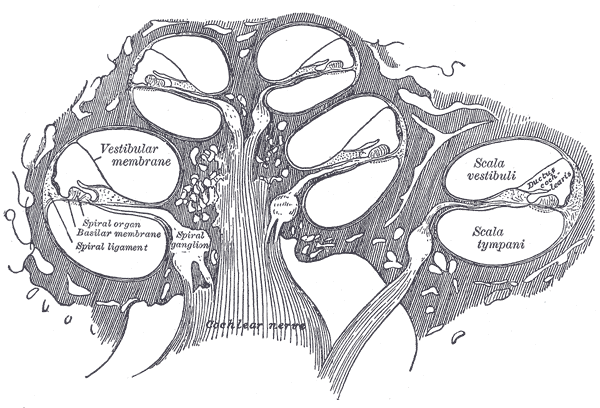
\includegraphics[width=\textwidth]{Gray928}
    \caption{Une représentation de la cochlée par Henry Vandyke Carter \& Henry Gray (1918) "Anatomy of the Human Body"} %  \url{https://commons.wikimedia.org/w/index.php?curid=566872}
  \end{marginfigure}

  Un autre élément d'importance est que la décomposition se fait sur une échelle logarithmique en fréquence et en amplitude . Le fait que l'amplitude d'un son soit perçue de manière logarithmique est relativement bien comprise, ce qui n'est pas le cas de l'axe fréquentiel. Des arguments d'ordre mathématique seront donnés à ce sujet dans la section dédiée au \lnameref{sec:scattering}.

  Il est important de noter que la communication entre le cortex auditif et la cochlée est bi directionnelle. De l'information est transmise de la cochlée vers le cortex auditif (direction montante) et du cortex vers la cochlée (direction descendante). Dans le cadre de la psycho perception, la direction montante est relativement aisément étudiable. Un sujet est soumis à un stimuli et doit répondre de manière plus ou moins explicite à des questions sur son expérience. La direction descendante est beaucoup plus difficile à étudier car elle implique de conditionner le sujet et de mesurer l'impact de ce conditionnement sur la performance de l'organe de réception lui même. Cela implique nécessairement une approche \og neuroscience \fg beaucoup plus invasive et complexe à mettre en \oe\~uvre comme celle effectuée par Nima Mesgarani avec des êtres humains, montrant l'importance de ces connexions descendantes et leurs capacités à conditionner la sensibilité du système auditif\cite{mesgarani2012selective}.

  A la fin du siècle dernier, les outils à disposition étant moins avancés qu'aujourd'hui, on questionnait essentiellement la perception et la cognition humaine par des approches \og holistiques \fg qui étudiaient nos réactions à des stimulis sans pour autant investiguer l'implantation effective dans le cerveau des mécanismes responsables de ces réactions.

  Pour le traitement du son, on s'accorde pour considérer que de nombreux éléments structurants sont communément utilisés par le sah pour inférer une représentation informative de la scène sonore auquel il est soumis. Pour les besoins de l'exemple, on représentera ici la sortie de la cochlée comme d'un spectrogramme ou encore d'un scalogramme. Un scalogramme est un spectrogramme dont les échelles de fréquences et d'amplitude sont logarithmiques. Ces représentations permettent de décomposer le signal sonore sur la plan temps / fréquence d'une manière fonctionnellement équivalente à la cochlée\footnote{Les détails de la construction du spectrogramme sont donnés dans la section dédiée au \lnameref{sec:tf}}. Du point de vue physiologique, ces représentations sont une grossière approximation~\cite{lyon2017human} mais elles constituent des références dans le domaine du traitement du signal sonore et c'est donc celles là que nous utiliserons ici.

  \begin{figure*}
    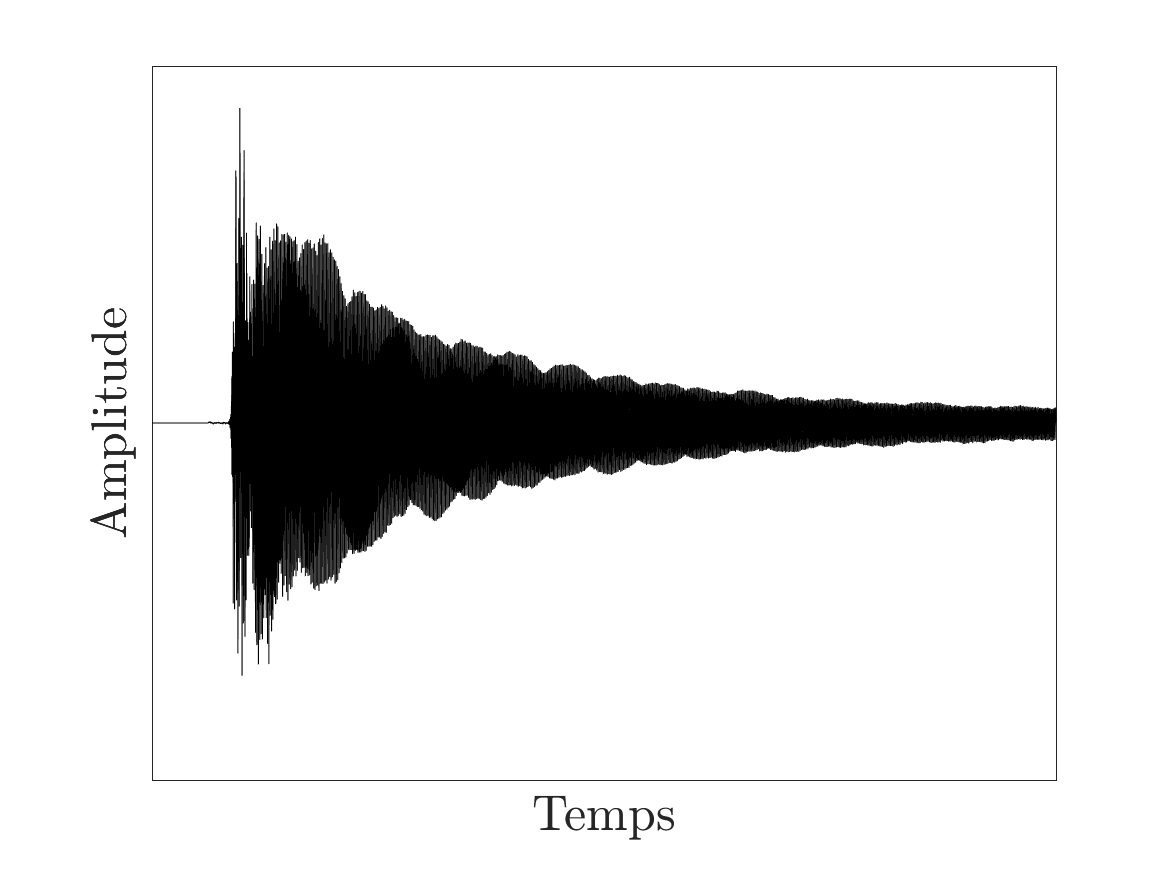
\includegraphics[width=.333\textwidth]{pianoGray}
    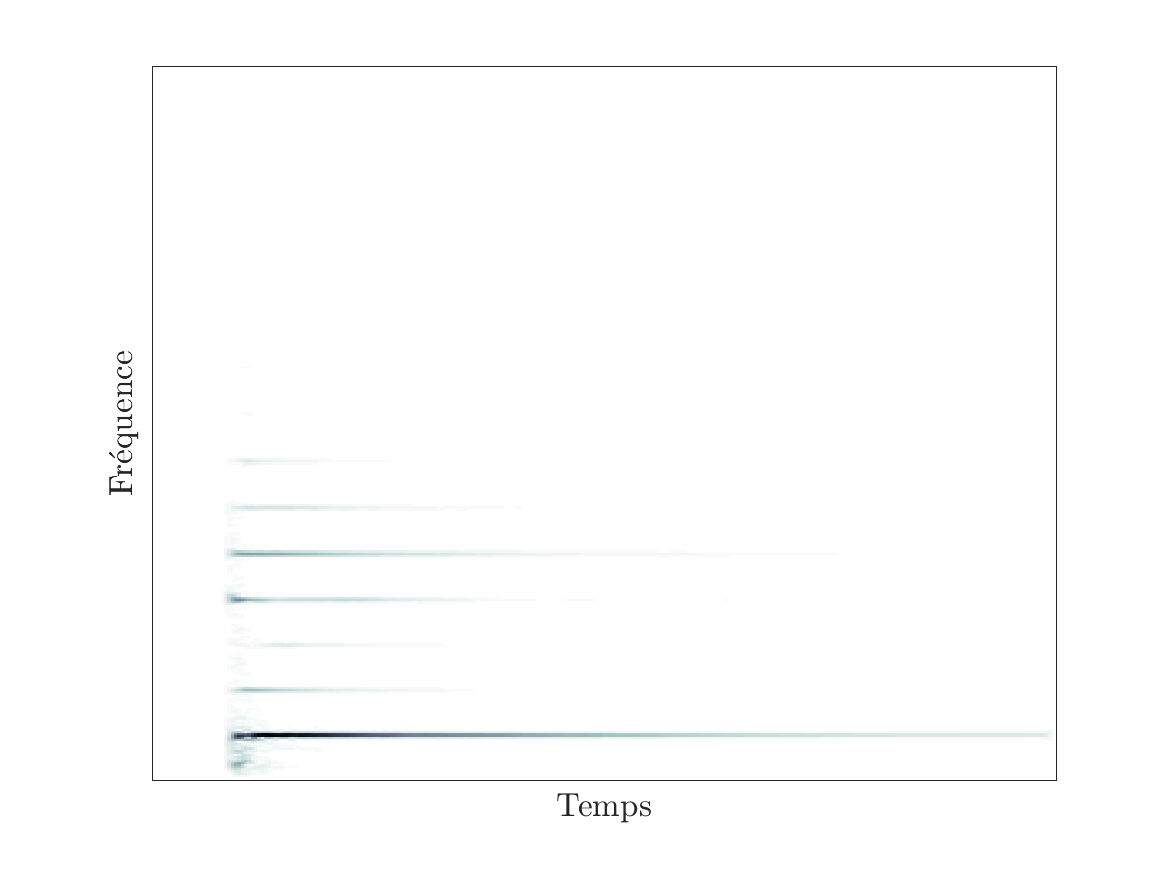
\includegraphics[width=.333\textwidth]{pianoSpec}
    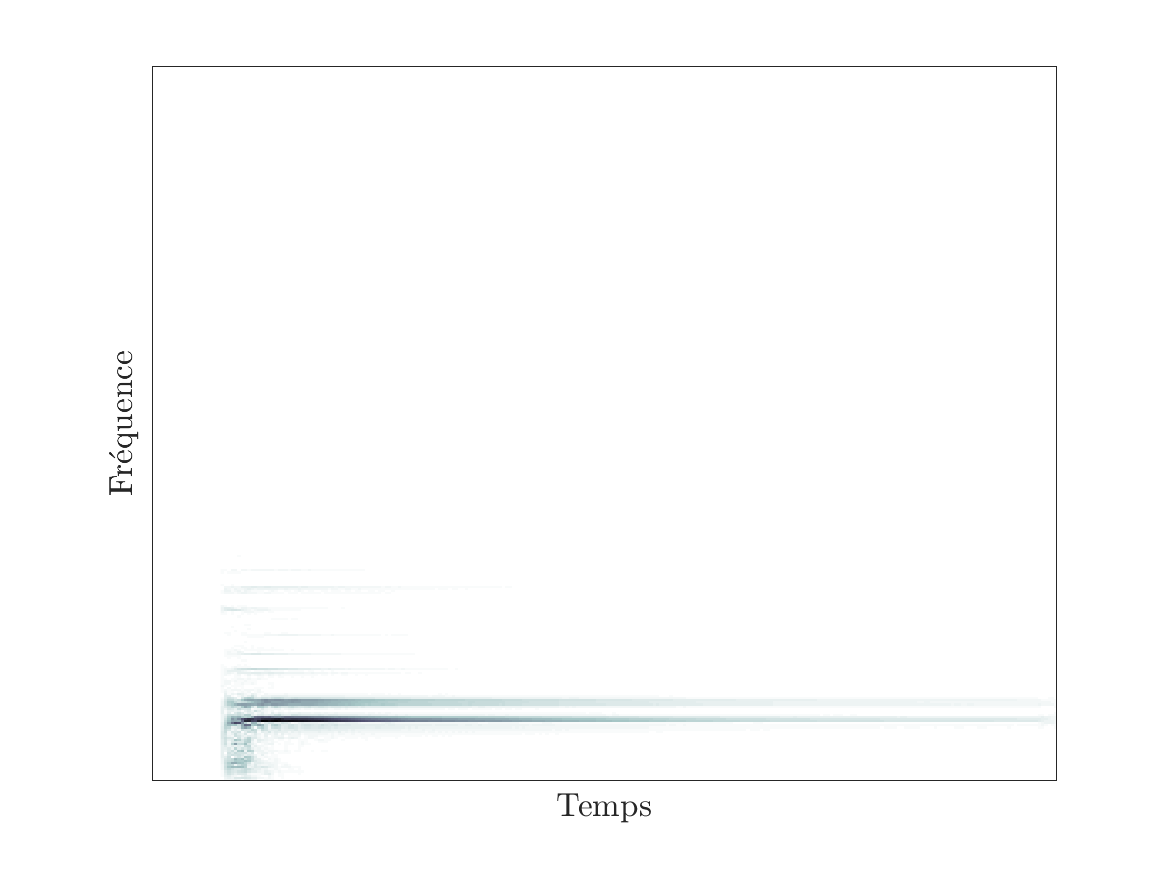
\includegraphics[width=.333\textwidth]{pianoScal}
    \caption{De gauche à droite, signal temporel, spectrogramme et scalogramme d'une note de piano.}
    \label{fig:piano}
  \end{figure*}

  Les traitements subséquents  du sah peuvent alors être approximés par une opération de segmentation du plan temps/fréquence en des sources données, et ce en fonction de certains critères.  On citera, dans l'ordre d'importance communément admis, l'harmonicité, la synchronicité, la proximité en fréquence, en temps, la rythmicité, etc. Par exemple, la Figure \ref{fig:piano} montre le spectrogramme d'une note de piano. Même si différentes résonances apparaissent comme disjointes sur le plan temps/fréquence nous ne percevons qu'une seule entité sonore. C'est bien qu'il y a eu un processus de formation de source, impliquant majoritairement ici le critère d'harmonicité. L'importance relative de ces critères dans ce processus de formation de sources peut être modulée dans une certaine mesure par des processus descendants comme l'attention ou encore la pratique\marginnote{\begin{center}
    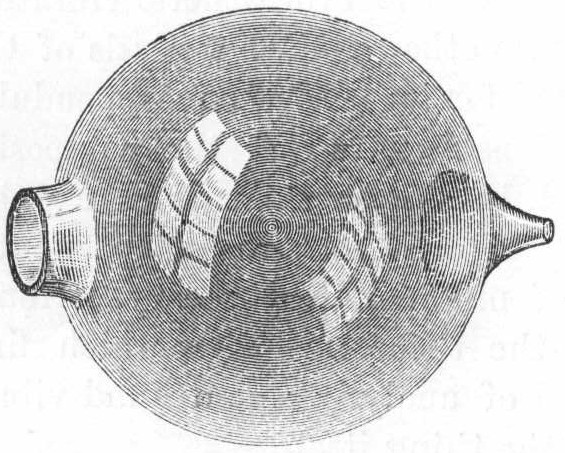
\includegraphics[width=.5\textwidth, angle =270]{resonatorCrop}
  \end{center}

   Helmholtz se disait capable de dissocier les différentes harmoniques d'une note de violon grâce à l'écoute répétée du son de ses résonateurs qui par leur dimensions judicieusement choisies permettaient d'implanter un filtre passe bande dont la fréquence centrale coïncidait avec la fréquence de certaines harmoniques des notes jouées.}.


  De nombreux autres indices ont été étudiés et de nombreux modèles de perception holistiques se basant sur les règles de la gestalt ont été proposés. En formalisant ces concepts dans une théorie unifiée, appuyée par de nombreuses expériences perceptives, Bregman a fondé l'analyse de scènes auditives (asa)\cite{bregman1994auditory}. Ces travaux ont suscités un élan d'intérêt dans la communauté traitement du signal et plusieurs modèles computationels ont été proposés comme celui de Dan Ellis\cite{ellis1996prediction}, pionnier dans ce domaine communément appelé casa, pour "computational auditory scene analysis".

  %En considérant le spectrogramme comme notre représentation de départ\marginnote{On néglige donc ici la notion de phase, comme cela est effectué dans la plupart des méthodes de séparation de sources.}, en simplifiant un peu les choses,

Suivant le principe de formation de sources de l'asa, on peut considérer que le problème casa consiste à attribuer automatiquement une couleur à chaque point du plan temps/fréquence, chaque couleur correspondant à une des sources d'intérêt. La figure \ref{fig:ibm}, montre le cas du masque binaire idéal dans le cas d'un mélange de deux sources sonores, une source harmonique (piano) et une source percussive (batterie). La partie sombre (structure verticale) correspond aux zones du plan temps / fréquence où la source percussive est dominante, la partie blanche (structure horizontale) correspond à la source harmonique. Ces masques sont dits idéaux parce qu'ils sont calculés grâce à la comparaison avec les spectrogrammes des sources avant mélange. Le masque binaire idéal est donc communément utilisé comme référence dite \og oracle \fg, car elle nécessite des connaissances dont le système casa que nous cherchons à évaluer ne dispose pas, ici les spectrogramme des sources avant mélange.

  \begin{figure*}
    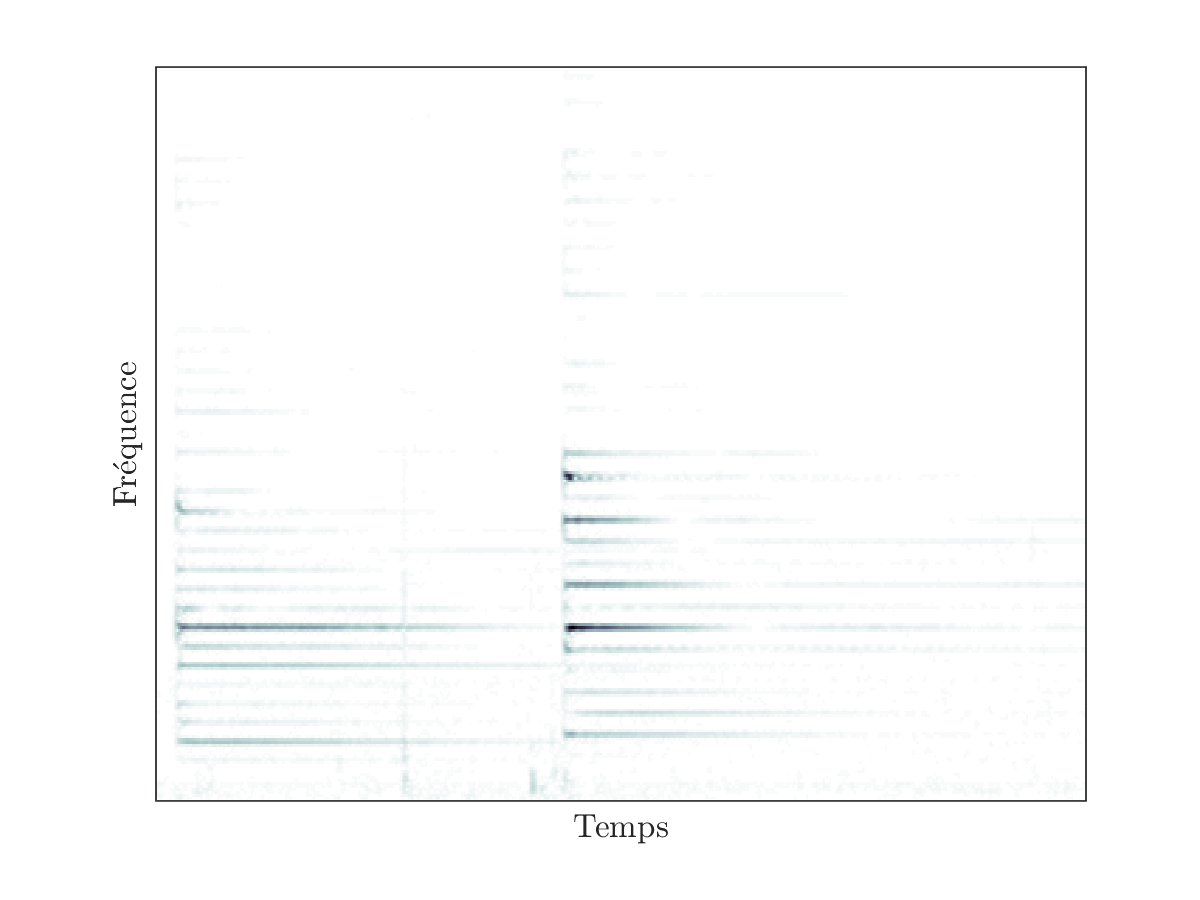
\includegraphics[width=.333\textwidth]{ibmB}
    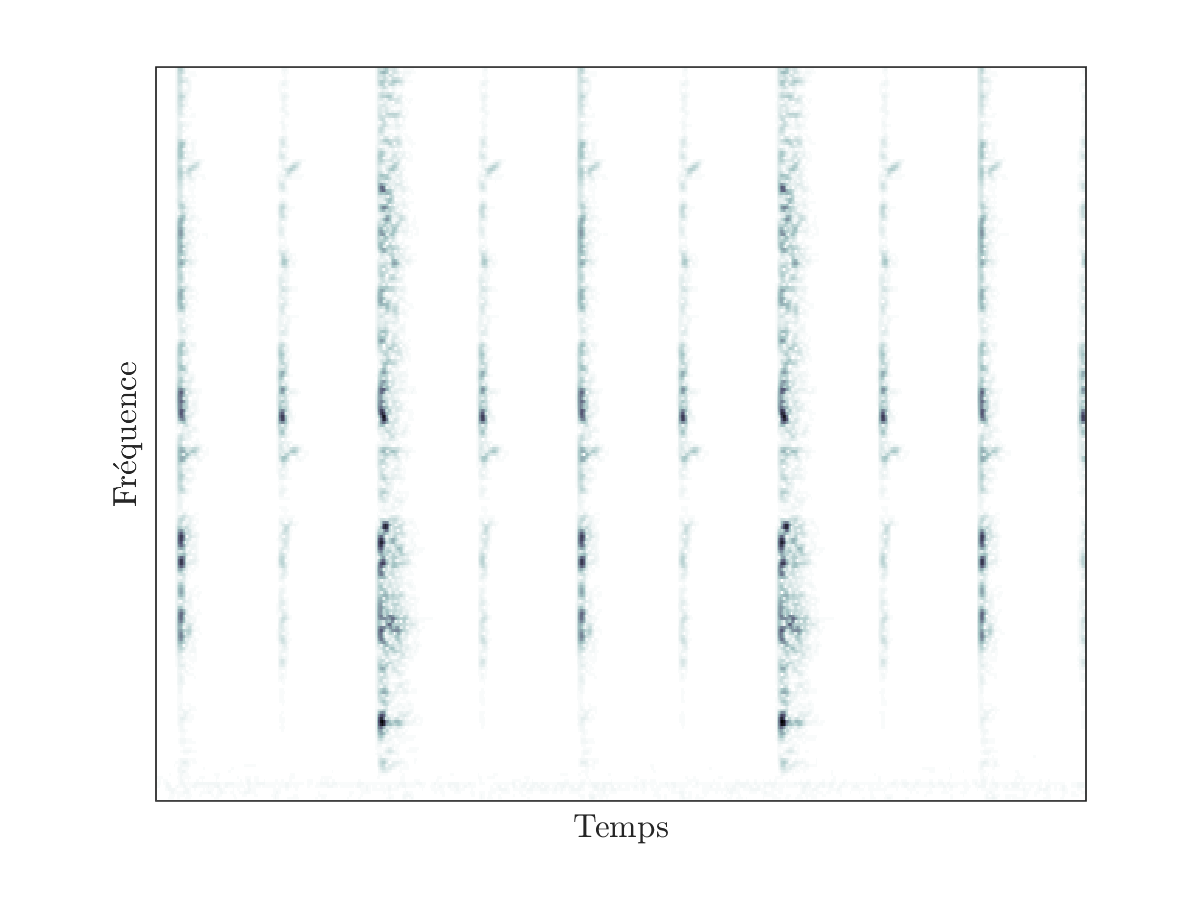
\includegraphics[width=.333\textwidth]{ibmA}
    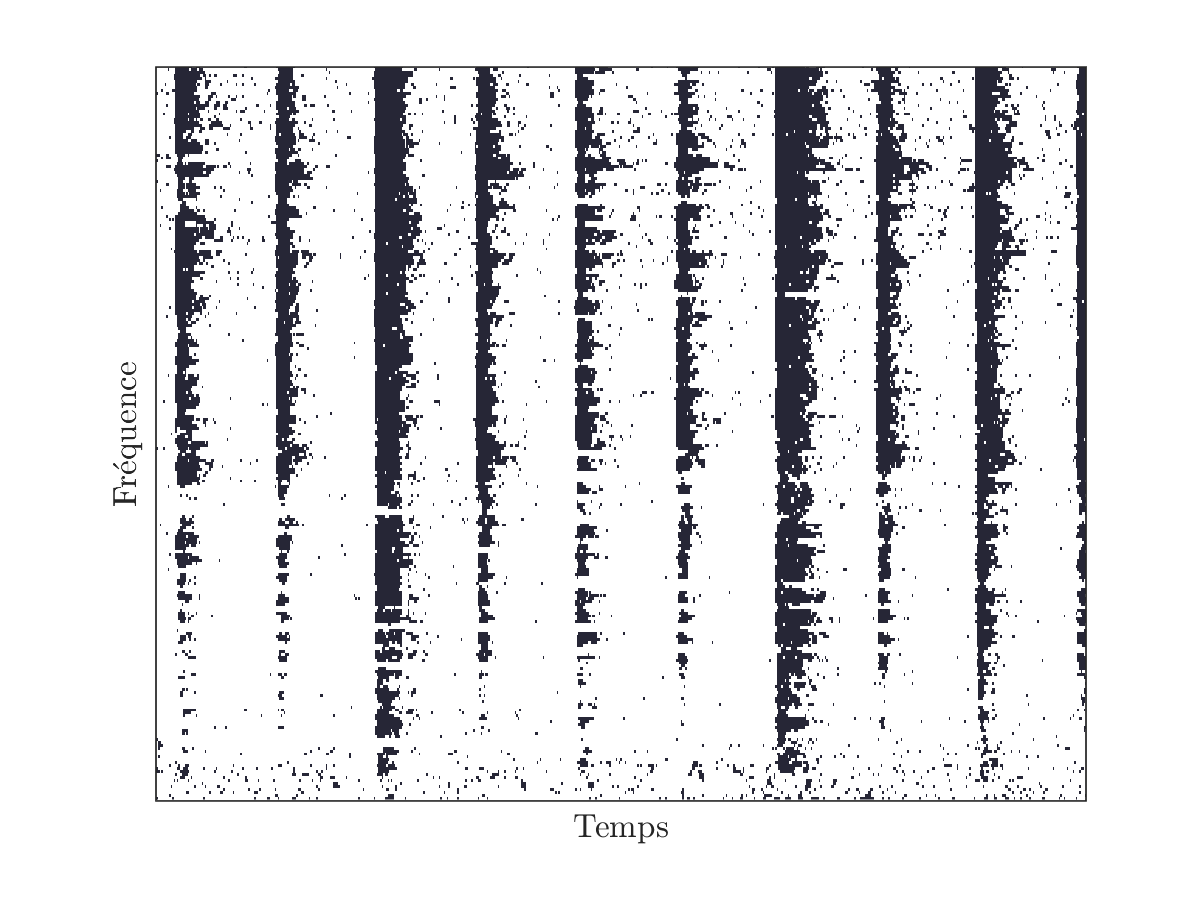
\includegraphics[width=.333\textwidth]{ibm}
    \caption{Spectrogrammes d'une source harmonique (piano), d'une source percussive (batterie) et masque binaire idéal correspondant.} \label{fig:ibm}
  \end{figure*}

  \subsection{Algorithmes de partitionnement}

  Séduit par l'aspect neuro-inspiré et la grande diversité algorithmique des approches casa, j'ai investi mon effort de recherche dans ce domaine en proposant plusieurs méthodes de segmentation du spectrogramme basés sur des algorithmes de regroupement d'objets, ou "clustering" en Anglais.

  Soit une scène sonore $S$ composée de plusieurs sources sonores $s_i$ représentée par un ensemble d'atomes temps/fréquence $a$ issue d'une décomposition du signal sonore donnée, on cherche alors à regrouper les atomes $a$ en fonction de leur appartenance aux sources $s_i$\footnote{Dans le cas d'une décomposition temps/fréquence comme le spectrogramme, les atomes seront les paniers temps / fréquence, indexés par leurs indices fréquentiels et temporels $a(t, f)$}. On supposera pour ce faire que la décomposition a été raisonnablement efficace, \textit{i.e.} $\forall a, \exists ! s_i | a \in s_i$. Comme on le voit sur la Figure~\ref{fig:ibm}, cette condition n'est pas complètement vérifiée dans le cas du spectrogramme car plusieurs paniers temps fréquence sont composés d'énergies des deux sources. On supposera alors que cette contamination est réduite et que cette condition est vérifiée pour un grand nombre d'atomes de grande énergie.

  Le problème casa peut alors se formaliser comme une procédure de regroupement d'atomes. Reste à 1) formaliser la procédure du regroupement, et 2) formaliser les critères asa. Pour formaliser la procédure de regroupement, on supposera maintenant la formalisation des critères asa effectuée, et disponible sous forme d'une notion de dissimilarité entre atomes : $$d(a_i, a_j) | d(a_i, a_j) < d(a_i, a_k) \text{si} \forall a_i, a_j \in s_i \text{et} \forall a_k \notin s_i$$.

  Le propos des algorithmes de regroupement est de trouver une partition d'un ensemble d'objets (ici des atomes temps/fréquence) en $K$ classes $C_k$ qui minimise la dissimilarité intra classe moyenne :
  \begin{equation}
    \argmin_{z_k} \sum_{k=1}^{K} z_k(i, j) d(a_i, a_j)
  \end{equation}
  où $z_k(i, j)$ est la fonction indicatrice de classe :
  \begin{equation}
    z_k(i, j)
    \begin{cases}
      1 \text{ si } a_i \text{ et } a_j \in C_k \\
      0 \text{ sinon}
    \end{cases}
  \end{equation}

  En supposant que $d$ définit un espace métrique comme c'est le cas d'une distance euclidienne appliquée à des objets décrits dans $\mathbb{R}^n$, l'algorithme des $k$-moyennes, proposé par Loyd\cite{lloyd1982least}, constitue la référence pour les problèmes de grande taille en nombre d'objets et d'un nombre de classe petit devant le nombre d'objet. Les relations casa que nous étudierons dans la suite n'étant pas exprimables sous forme d'une distance euclidienne, nous portons notre attention sur des algorithmes alternatifs, adaptés aux espaces non euclidiens.

  On peut par exemple formaliser le problème de regroupement comme un problème de partitionnement de graphe, où chaque objet constitue un n\oe{}ud et chaque dissimilarité pondère un arc entre deux n\oe{}uds. L'algorithme des "normalized cuts" permet de résoudre ce problème du regroupement d'objets. Cet algorithme a été popularisé dans le domaine de la segmentation d'image\cite{shi2000normalized}, où les pixels de l'image forment les n\oe{}uds du graphe et les arcs sont pondérés par proximité sur une échelle de gris avec contrainte de localité spatiale. Comme cela sera détaillé dans la section suivante, nous avons, en adaptant la formulation de ce poids aux critères asa, appliqué avec un certain succès cette approche au problème casa. Néanmoins, pour des problèmes de grande taille (en nombre d'atomes, comme en nombre de sources), une alternative à cet algorithme s'est révélée nécessaire. L'algorithme des coupures normalisées est en effet coûteux, principalement à cause d'une étape de décomposition en valeurs singulières d'une version transformée de la matrice de dissimilarité qui est de taille $n^2$ où $n$ est le nombre d'objets considérés. Dans le cas du problème casa, cela contraint fortement l'horizon temporel exploitable. Il nécessite également que la dissimilarité puisse s'exprimer comme un noyau pour garantir sa convergence, ce qui n'est pas le cas en général.

  Brian Kullis montre que l'objectif des coupures normalisées peut être formulé comme une fonction de coût optimisable par un algorithme de regroupement à noyau "kernel k-means", ce qui permet d'approcher le problème du regroupement par coupures normalisées avec une complexité considérablement réduite. Il reste que la convergence de ce type d'approche n'est vérifiée que dans le cas où la matrice de dissimilarité est semi définie positive. Il est possible de manipuler une matrice symétrique non semi définie positive pour la rendre semi définie positive\cite{optimal2003} mais l'impact de cette manipulation sur le regroupement obtenu est difficile à quantifier. Les relations casa étant complexes à modéliser et ne vérifiant pas en général cette contrainte, il nous a paru important de disposer d'un algorithme de regroupement efficace qui s'affranchisse de cette contrainte.

  Nous avons donc développé un algorithme de regroupement, nommé \textsl{k-averages}, dont la convergence est assurée pour tout type de matrice de dissimilarité, pour peut qu'elle soit symétrique, \textit{i.e.} $d(a, b) = d(b,a)$. Cette approche, même si elle considère des relations bien connues, n'avait, à notre connaissance, pas été complètement formalisée  en un algorithme effectif. Son évaluation sur un large ensemble de corpus\cite{UCRArchive} montre des performances équivalentes aux méthodes à noyau, avec un coût de calcul et une empreinte mémoire plus faible, ce qui la rend intéressante pour des problèmes de grande taille\cite{rossignol2018efficient}.

  \begin{figure*}[t]
    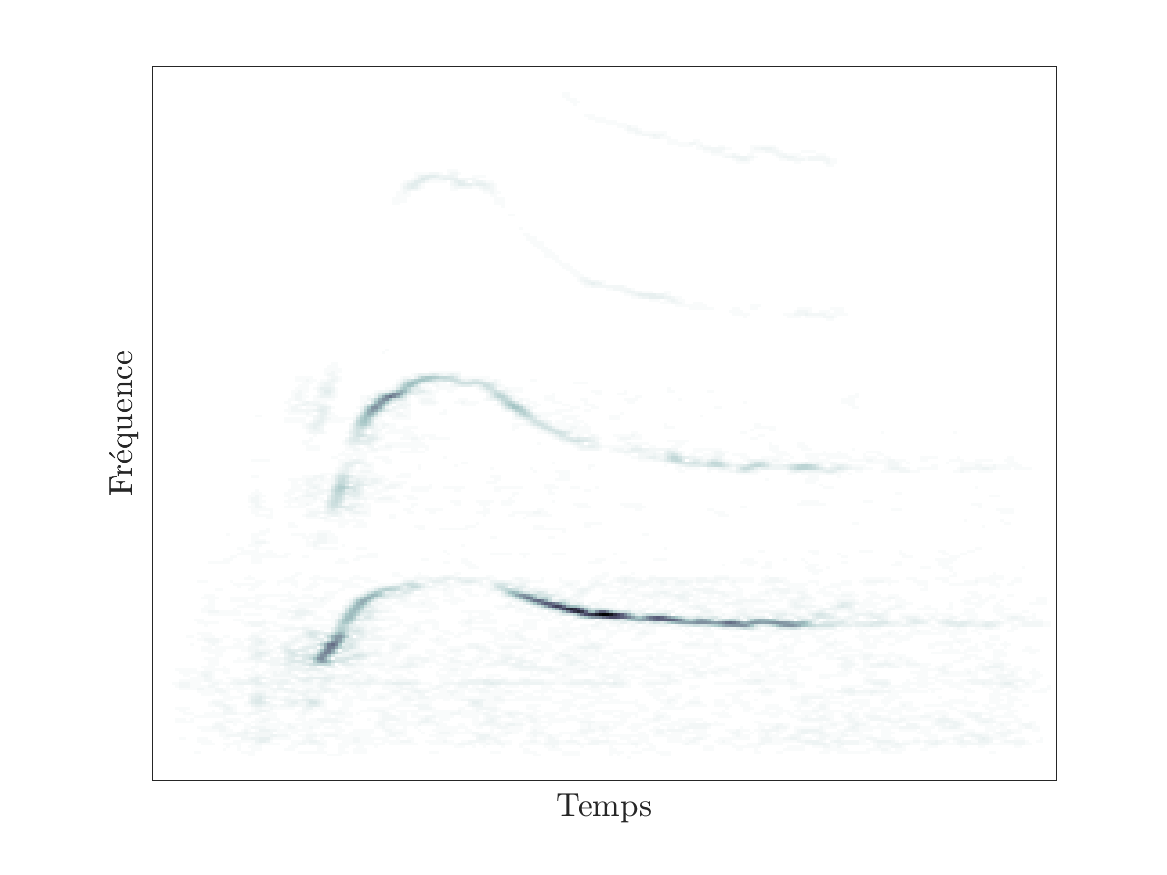
\includegraphics[width=.333\textwidth]{orcaOriSpec}
    \includegraphics[width=.333\textwidth]{orcaSin}
    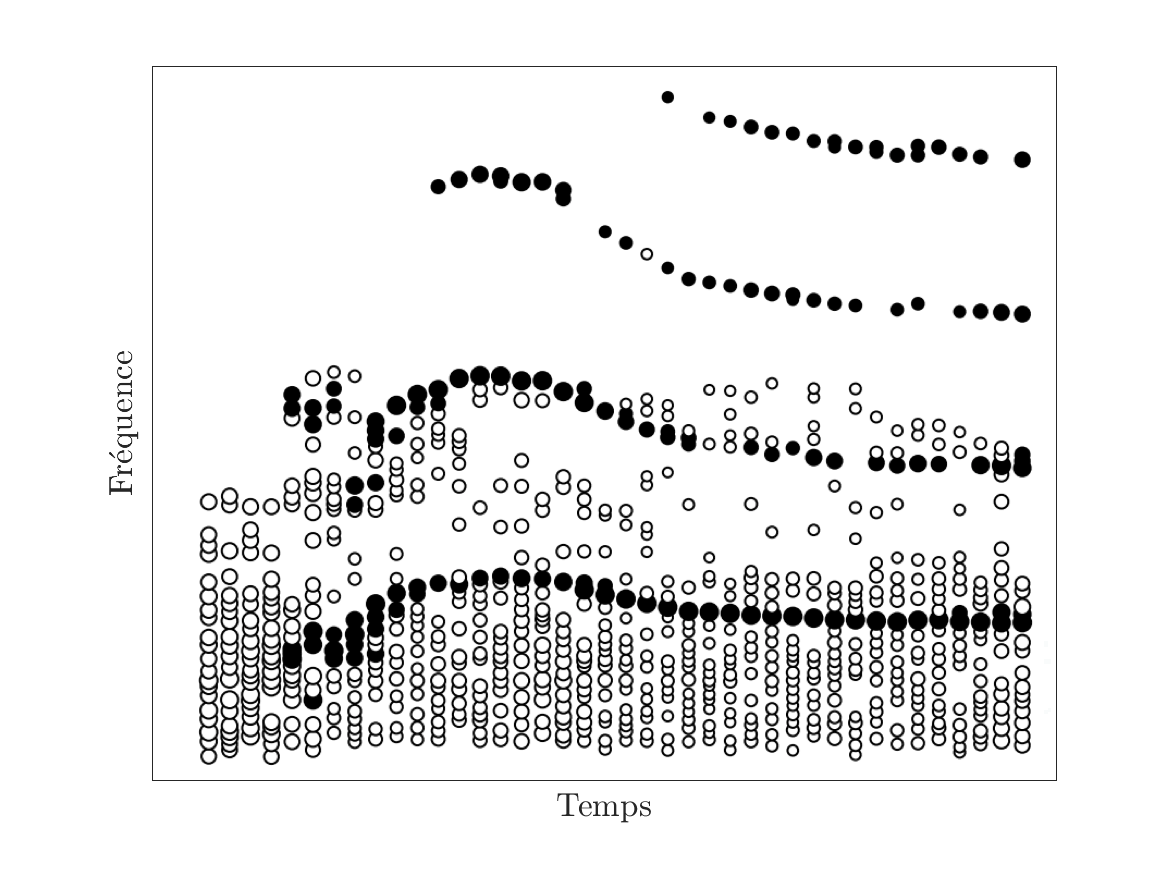
\includegraphics[width=.333\textwidth]{orcaSep}
    \label{fig:orca}
    \caption{Spectrogramme, représentation sinusoïdale à court terme et segmentation de cette représentation grâce à l'algorithme des coupures normalisées d'une vocalisation d'orque captée grâce à un hydrophone dans les eaux du "Inside passage" au nord de l'île de Vancouver, Colombie Britannique, Canada.}
  \end{figure*}

  \subsection{Applications au problème casa}

  % Soient deux pixels d'index $i$ et et $j$ décrits par une composante de gris $G \in \mathbb{R}$ et un vecteur de coordonées spatiales $X \in \mathbb{R}^2$, le poids $w(i, j)$ de l'arc reliant les pixels $i$ et $j$ s'exprime comme suit :
  % \begin{eqnarray}
  % w(i, j) &=& e^{\frac{-|G(i)-G(j)|^2}{\sigma^2_G}} \times \\
  % &&  \begin{cases}
  % e^{\frac{-|X(i)-X(j)|^2}{\sigma^2_X}} & \text{si} |X(i)-X(j)| < r, \\
  % 0 & \text{sinon}
  % \end{cases}
  % \label{eq:shi}
  % \end{eqnarray}

  Dans une première étude menée à l'Université de Victoria en collaboration avec George Tzanetakis, j'ai considéré le problème suivant : comment isoler la partie harmonique dominante d'un enregistrement polyphonique ?  Cela peut être le cas de vocalisations de mammifères marins, comme illustré avec la Figure \ref{fig:orca}, ou de la mélodie dans un enregistrement musical polyphonique.

  Soit une représentation sinusoïdale à court terme d'un signal sonore où chaque atome $A_l^k$ est paramétrisé par une fréquence $f_l^k$ et une amplitude $a_l^k$ et $k$ et $l$ désignent respectivement l'indice de trame et l'indice de l'atome au sein de la trame. \footnote{Une représentation sinusoïdale à court terme peut être considérée ici comme une version parcimonieuse et compacte du spectrogramme où l'on a identifié et modélisé les composantes de forte énergie par des sinusoïdes fenêtrées. Le lecteur peut se référer à la section dédiée à la modélisation basée sur des  \lnameref{sec:sct} pour plus de détails.}. Partant de cette représentation, le problème précité se formule comme suit : comment définir mathématiquement certaines relations asa pour ce type de représentation, les combiner entre elles, et en fonction de ces relations isoler la partie qui se conforme le plus aux critères exprimés ?



La Figure \ref{fig:ncut} donne le schéma fonctionnel du processus de segmentation\footnote{Son implantation a été diffusée dans l'environnement de traitement du signal audio Marsyas \url{http://marsyas.info}}. La contrainte de localité est ici exprimée en temps et de manière implicite par l'utilisation d'une fenêtre de "texture" composée de plusieurs trames. Cette approche permet de considérer un intervalle de temps suffisamment long tout en respectant des contraintes de complexité.

Les indices de proximité locale s'expriment en terme de fréquence et d'amplitude :
  \begin{equation}
  W_f \left( A _ { l } ^ { k } , A _ { m } ^ { k + n } \right) = e ^ { - \left( \frac { f _ { l } ^ { k } - f _ { m } ^ { k + n } } { \sigma _ { f } } \right) ^ { 2 } }
  \end{equation}
  \begin{equation}
  W_a \left( A _ { l } ^ { k } , A _ { m } ^ { k + n } \right) =  e ^{ - \left( \frac { a _ { l } ^ { k } - a _ { m } ^ { k + n } } { \sigma _ { a } } \right) ^ { 2 } }
  \end{equation}
  où $\sigma _ { f }$ et $\sigma _ { a }$ permettent de contrôler l'importance relative des deux facteurs dans la mesure de proximité finale.

  \begin{figure}[t]
          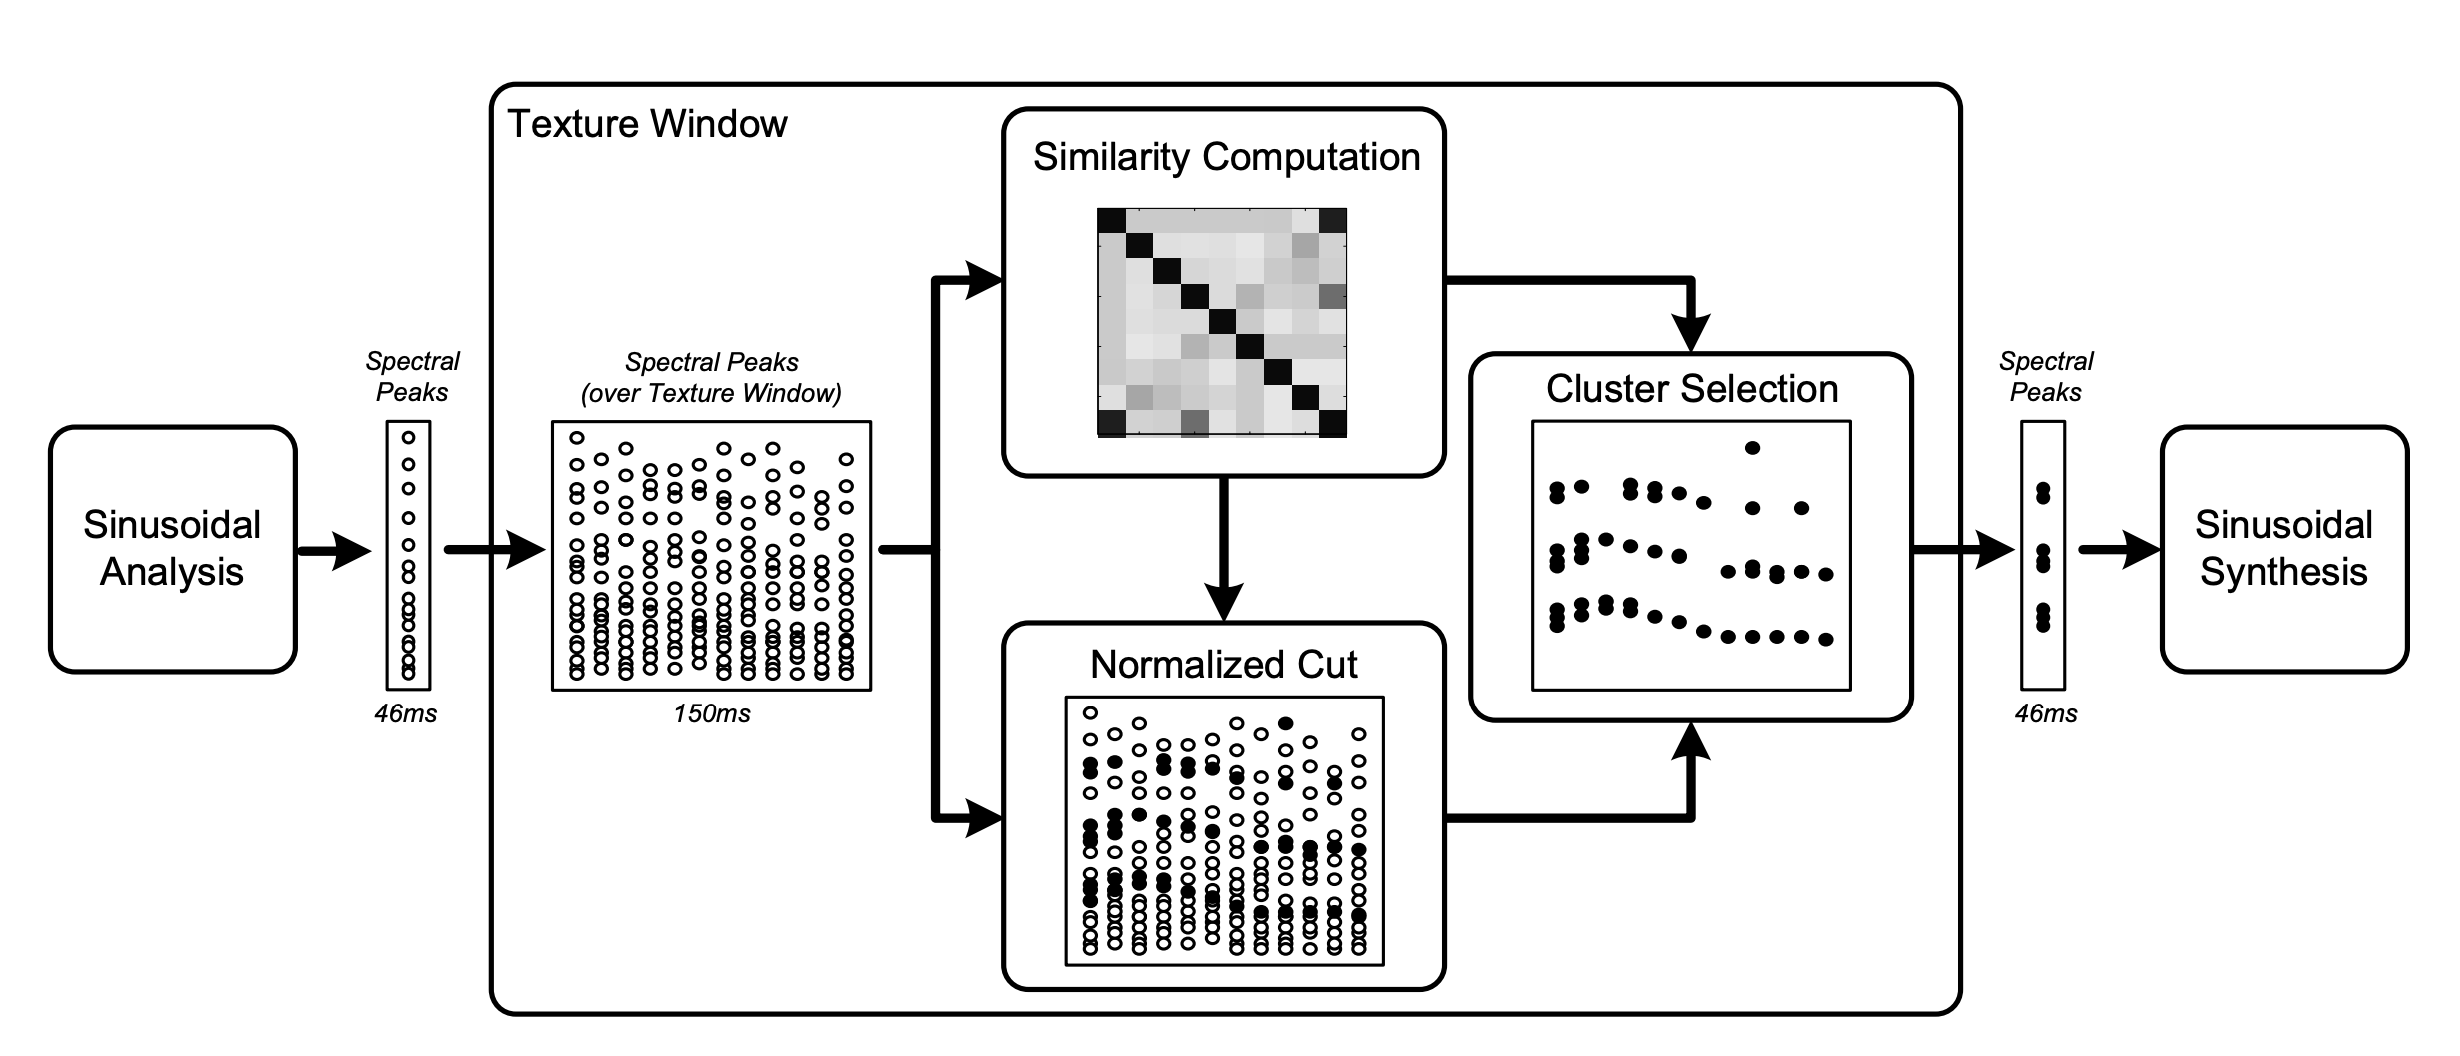
\includegraphics[width=1\textwidth]{figures/ncutDiagram.png}
        \caption{Schéma fonctionnel du processus de segmentation basé sur l'algorithme des coupures normalisées.}  \label{fig:ncut}
\end{figure}

  En revanche la relation d'harmonicité potentiellement entretenue entre deux atomes ne peut s'exprimer de manière robuste d'une manière aussi directe. En effet, le fait que les fréquences des deux atomes considérés soient en relation harmonique n'est pas une condition suffisante pour exprimer le fait que ces deux atomes appartiennent à une source harmonique. Pour palier à ce problème, nous assignons à chaque atome, un profil harmonique composé à partir de l'ensemble des atomes présents dans la même trame. Ce profil est ensuite judicieusement manipulé pour maximiser la probabilité d'un bon alignement de ces profils si les deux atomes appartiennent à la même source harmonique\cite{lagrangeTaslp08}. Le critère s'exprime alors comme une corrélation entre ces deux profils :
  \begin{equation}
   { W _ { h } \left( A _ { l } ^ { k } , A _ { m } ^ { k + n } \right) = e \left( \frac { c _ { \left( H _ { l } ^ { k } , H _ { m } ^ { k + n } \right) } } { \sqrt { c \left( H _ { l } ^ { k } , H _ { l } ^ { k } \right) \cdot \left( H _ { m } ^ { k + n } , H _ { m } ^ { k + n } \right) } } \right) ^ { 2 } }
  \end{equation}
  où
  \begin{equation}
    { c \left( H _ { a } ^ { b } , H _ { c } ^ { d } \right) = \sum _ { i } H _ { a } ^ { b } ( i ) * H _ { c } ^ { d } ( i ) }
  \end{equation}
  La segmentation effectuée grâce à la combinaison de ces trois critères $W = W_a W_f W_h$ permet d'isoler un certain nombre de parties dans chaque fenêtre de texture. La partie la plus "dense" dans l'espace de représentation est ensuite sélectionnée. Soit un ensemble d'atomes d'une même classe
  $$C _ { d } = \left\{ A _ { m } ^ { k } | \operatorname { label } \left( A _ { m } ^ { k } \right) = c \right\}$$,
  ce critère de densité s'exprime comme suit :
  \begin{equation}
  d \left( C _ { d } \right) = \frac { 1 } { \# C _ { d } ^ { 2 } } \sum _ { A _ { l } ^ { k } \in C _ { d } } \sum _ { a _ { m } ^ { j } \in C _ { d } } W _ { f a h } \left( A _ { l } ^ { k } , A _ { m } ^ { j } \right)
  \end{equation}

  % \begin{figure}[t]
  %         \includegraphics[width=1.2\textwidth]{figures/orcaSin.png}
  %        \caption{Segmentation d'un modèle sinusoïdal à court terme calculé à partir d'un enregistrement de vocalisation d'orque. Les points noirs correspondent aux atomes du cluster de densité maximale.}\label{fig:orca}
  % \end{figure}



Ce premier système m'a permis d'explorer des critères de type instantanés, \textit{i.e.} locaux en temps. Au sein de l'Ircam, et en collaboration avec Mathias Rossignol, je me suis focalisé sur la notion de structure séquentielle, en faisant le postulat suivant : toute segmentation est effectuée sur la base de contraintes de localité dans deux espaces conceptuellement disjoints mais complémentaires : un espace analogue à l'espace/temps, et un autre relatif à une notion de forme. Ces deux types d'espaces de représentation induisent respectivement des relations 1) de proximité et de continuité, et 2) de similarité; leur composition amenant une autre notion, la notion de structure. Précisons le propos : %Prenons l'exemple d'une cuillère à café placée dans une tasse et une cuillère à soupe placée plus loin sur une table. La cuillère à café étant dans la tasse, elle est proche spatialement de la tasse, et elle est également similaire à la cuillère à soupe située un peu plus loin.

\begin{enumerate}
\item la continuité signifie que nous identifions de préférence comme des objets des fragments sonores sans rupture,
\item la similitude signifie qu'en cas de rupture de l'objet, tous ses composants doivent néanmoins partager des propriétés spectrales communes, puisqu'elles sont produites par une même source,
\item la notion de  structure, enfin, reflète la manière dont les auditeurs peuvent reconnaître des objets complexes en identifiant des motifs répétés : par exemple, des sons mécaniques complexes ou des appels d'animaux peuvent être constitués de plusieurs fragments non continus et dissimilaires, mais la répétition de ces formes permet d'en identifier la structure.
\end{enumerate}

L'utilisation conjointe de ces contraintes est particulièrement difficile à formaliser, mais néanmoins indispensable à l'obtention d'une segmentation de qualité. Le schéma fonctionnel de la Figure \ref{fig:alc}, montre comment ces axes de structuration ont été considérés.

%Un exemple de composition de trouve dans le critère utilisé en segmentation d'image par Shi \& al, comme on le voit dans l'équation \ref{eq:shi}, on peut, dans le cas de la segmentation d'une image, définir la notion de similarité par une différence de colorimétrie entre les deux pixels comparés. La notion de proximité introduit elle une notion de seuil.

En partant d'objets élémentaires comme le pixel d'une image ou le panier temps / fréquence d'un spectrogramme, il est évident que la notion de proximité doit prédominer, car les notions de similarité et \textit{à fortiori} le critère de séquentialité se basent alors sur une quantité d'information trop réduite.  En revanche, plus on considère des objets complexes, plus cette tendance va s'inverser. Fort de ce constat, nous avons donc chercher à concevoir un algorithme de structuration hiérarchique basé sur l'expression de ces critères qui soit adapté à la segmentation de scènes sonores\cite{rossignolhal-01122006}.


\begin{figure}[t]
        
\includegraphics[width=1\textwidth]{figures/alc_one_level.png}
       \caption{Schéma décrivant les principaux traitements utilisés pour passer du niveau $i$ au suivant. Une étape de classification non supervisée des fragments $o_i$ produit des labels $c_i$ qui sont utilisés comme information structurelle, qui combinée avec un critère de continuité spectrale, guide la détermination des fragments $o_{i+1}$ du niveau suivant.}\label{fig:alc}
\end{figure}

L'algorithme proposé effectue un regroupement hiérarchique ascendant des trames d'un spectrogramme. La première étape ne considère que le  critère de continuité, \textit{i.e.} une similarité sous contrainte de localité. Cette étape permet d'avoir des fragments plus spécifiques, un élément important pour obtenir une mesure de séquentialité qui soit pertinente dès le début du processus de structuration. Pour les niveaux suivants, on considère la combinaison d'une mesure de similarité de forme, exprimée comme le coût minimal d'un alignement élastique entre les deux fragments comparés, et d'une mesure de similarité de séquence, calculée à partir d'une quantification des trames associées aux fragments. L'algorithme procède comme suit :


  \begin{enumerate}
  \item \textbf{Initialisation} par une première classification : regrouper les trames successives qui ont une grande similarité spectrale pour déterminer les fragments de niveau 0
  \item \textbf{Répéter} pour le nombre spécifié de niveaux :
    \begin{itemize}
    \item Calcul des similarités entre fragments de niveau $i$
    \item Classifier ces fragments en classes $C_i$ en fonction de ces similarités
    \item Calcul de l'information mutuelle entre les $C_i$, en se basant sur le degré de séquentialité entre $C_i$ et $C_j$ :
      \[ MI \left( C_i, C_j \right) = \log \left(\frac{p\left(C_iC_j\right)}{p\left(C_i\right)p\left(C_j\right)}\right) \]
      où $p(C)$ désigne la probabilité qu'un fragment appartienne à une classe donnée, et $p(C_iC_j)$ est la probabilité que deux éléments soient consécutifs.
    \item Générer une courbe de décision le long de l'axe temporel fonction de:
      \begin{itemize}
      \item l'information mutuelle entre les classes des deux fragments consécutifs,
      \item la continuité spectrale, définie comme la similarité spectrale entre la fin d'un fragment et le début du fragment suivant.
        \end{itemize}
    \item Segmenter la séquence de fragments en fonction de la courbe de décision, en combinant les fragments situés entre les minima locaux de cette courbe de décision.
    \end{itemize}
  \end{enumerate}

  % \begin{figure}[t]
  %         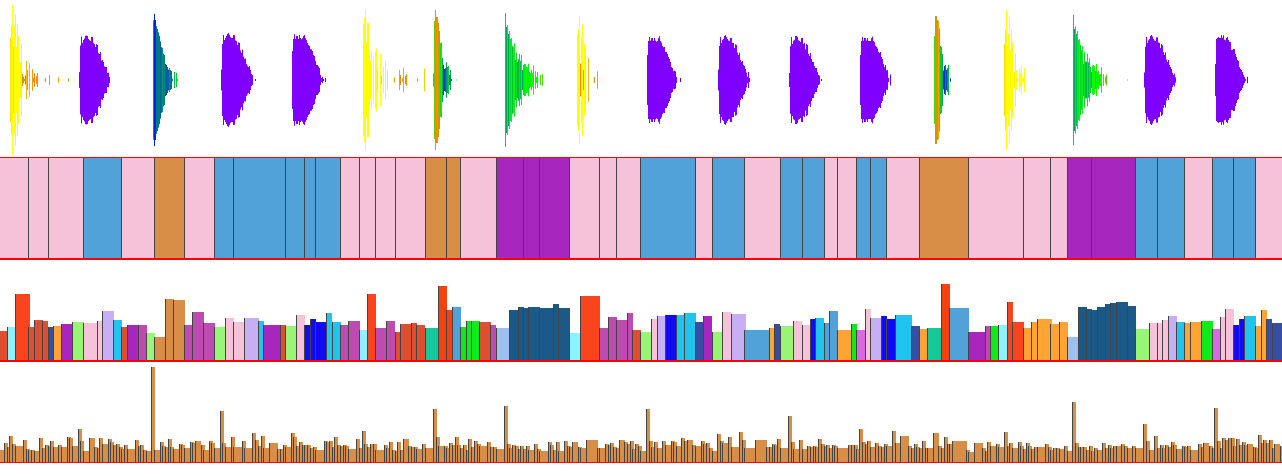
\includegraphics[width=\textwidth]{figures/alc_sample}
  %        \caption{Exemple de segmentation obtenue. La forme d'onde est donnée pour référence avec un code couleur correspondant à sa hauteur. A chaque niveau, la largeur des blocs indique le support temporel du fragment associé, la hauteur indique la valeur de la fonction de décision à ce niveau, et la couleur le label associé à la classe à laquelle le fragment appartient.}  \label{fig:alcéchantillon}
  % \end{figure}

%La Figure~\ref{fig:alcéchantillon} montre un exemple de segmentation obtenue en considérant une séquence de batterie. Au niveau le plus bas (bas de la figure), de très petits fragments sont regroupés en unités plus cohérentes. Au niveau intermédiaire, les fragments sont encore très petits, mais suffisamment grands pour être regroupés de manière assez significative. Au niveau supérieur, les événements correspondants aux notes jouées et les fragments sont regroupés en fonction du type d'objet auquel ils appartiennent. Dans cet exemple, la configuration de l'algorithme conduit à une sur-segmentation du signal et, au dernier niveau, le regroupement identifie correctement les hits charleston (classe bleue) et distingue deux types de hits de caisse claire (classes orange et violette) ce qui se vérifie effectivement à l'oreille et visuellement en fonction du code couleur associé au signal temporel. En revanche, la grosse caisse (en jaune sur le signal) est confondue avec le fond sonore (classe rose pâle).

La Figure~\ref{fig:smoke} présente la segmentation de l'introduction du célèbre morceau de Deep Purple \emph{Smoke on the Water}. La même phrase musicale est répétée deux fois avec quelques variations d'interprétation. Des motifs émergent à partir du niveau 4 où les motifs élémentaires du riff sont révélés.

\subsection{Constat}

  Ces années d'exploration des approches casa m'ont permises de parcourir de larges champs d'expertise scientifiques, de l'informatique au traitement du signal, de la psycho-perception aux neurosciences, mais cela a surtout été pour moi l'occasion de mieux saisir l'importance de certaines problématiques fondamentales en sciences des données :
  \begin{enumerate}
    \item Comment dévoiler la structure intrinsèque aux données à partir d'observations bruitées ?
    \item Comment exploiter l'approche compositionnelle de notre compréhension du monde ?
    \item Quel rôle peut jouer la notion de mémoire dans les processus pré-cités ?
  \end{enumerate}
  Ces questions continuent de nourrir mes recherches car les solutions auxquelles j'ai contribué ne sont en aucun cas satisfaisantes. La traduction algorithmique de contraintes de structuration est un art difficile, car elle nécessite un effort important pour fiabiliser les algorithmes. La gestion de l'interaction entre les différentes contraintes de structuration l'est aussi. Enfin, la notion de mémoire est ici exploitée de manière implicite en considérant la redondance d'information dans la scène observée. Avec les horizons temporels considérés à l'époque pour rendre l'approche tractable, cette approche s'est révélé insuffisante.  %L'utilisation d'un schéma alterné dans l'algorithme alc a permit de mieux contrôler cette interaction mais cela reste au fond arbitraire.

  Au delà de ces problématiques propres aux approches casa, les approches de séparation de sources se basent généralement sur un traitement en deux temps : 1) représentation du signal audio sous forme de spectrogramme, 2) segmentation. On verra dans le chapitre dédié à la \lnameref{chap:modeles}, les limites ce que cela impose sur la performance de ces approches.


    \begin{figure}[t]
            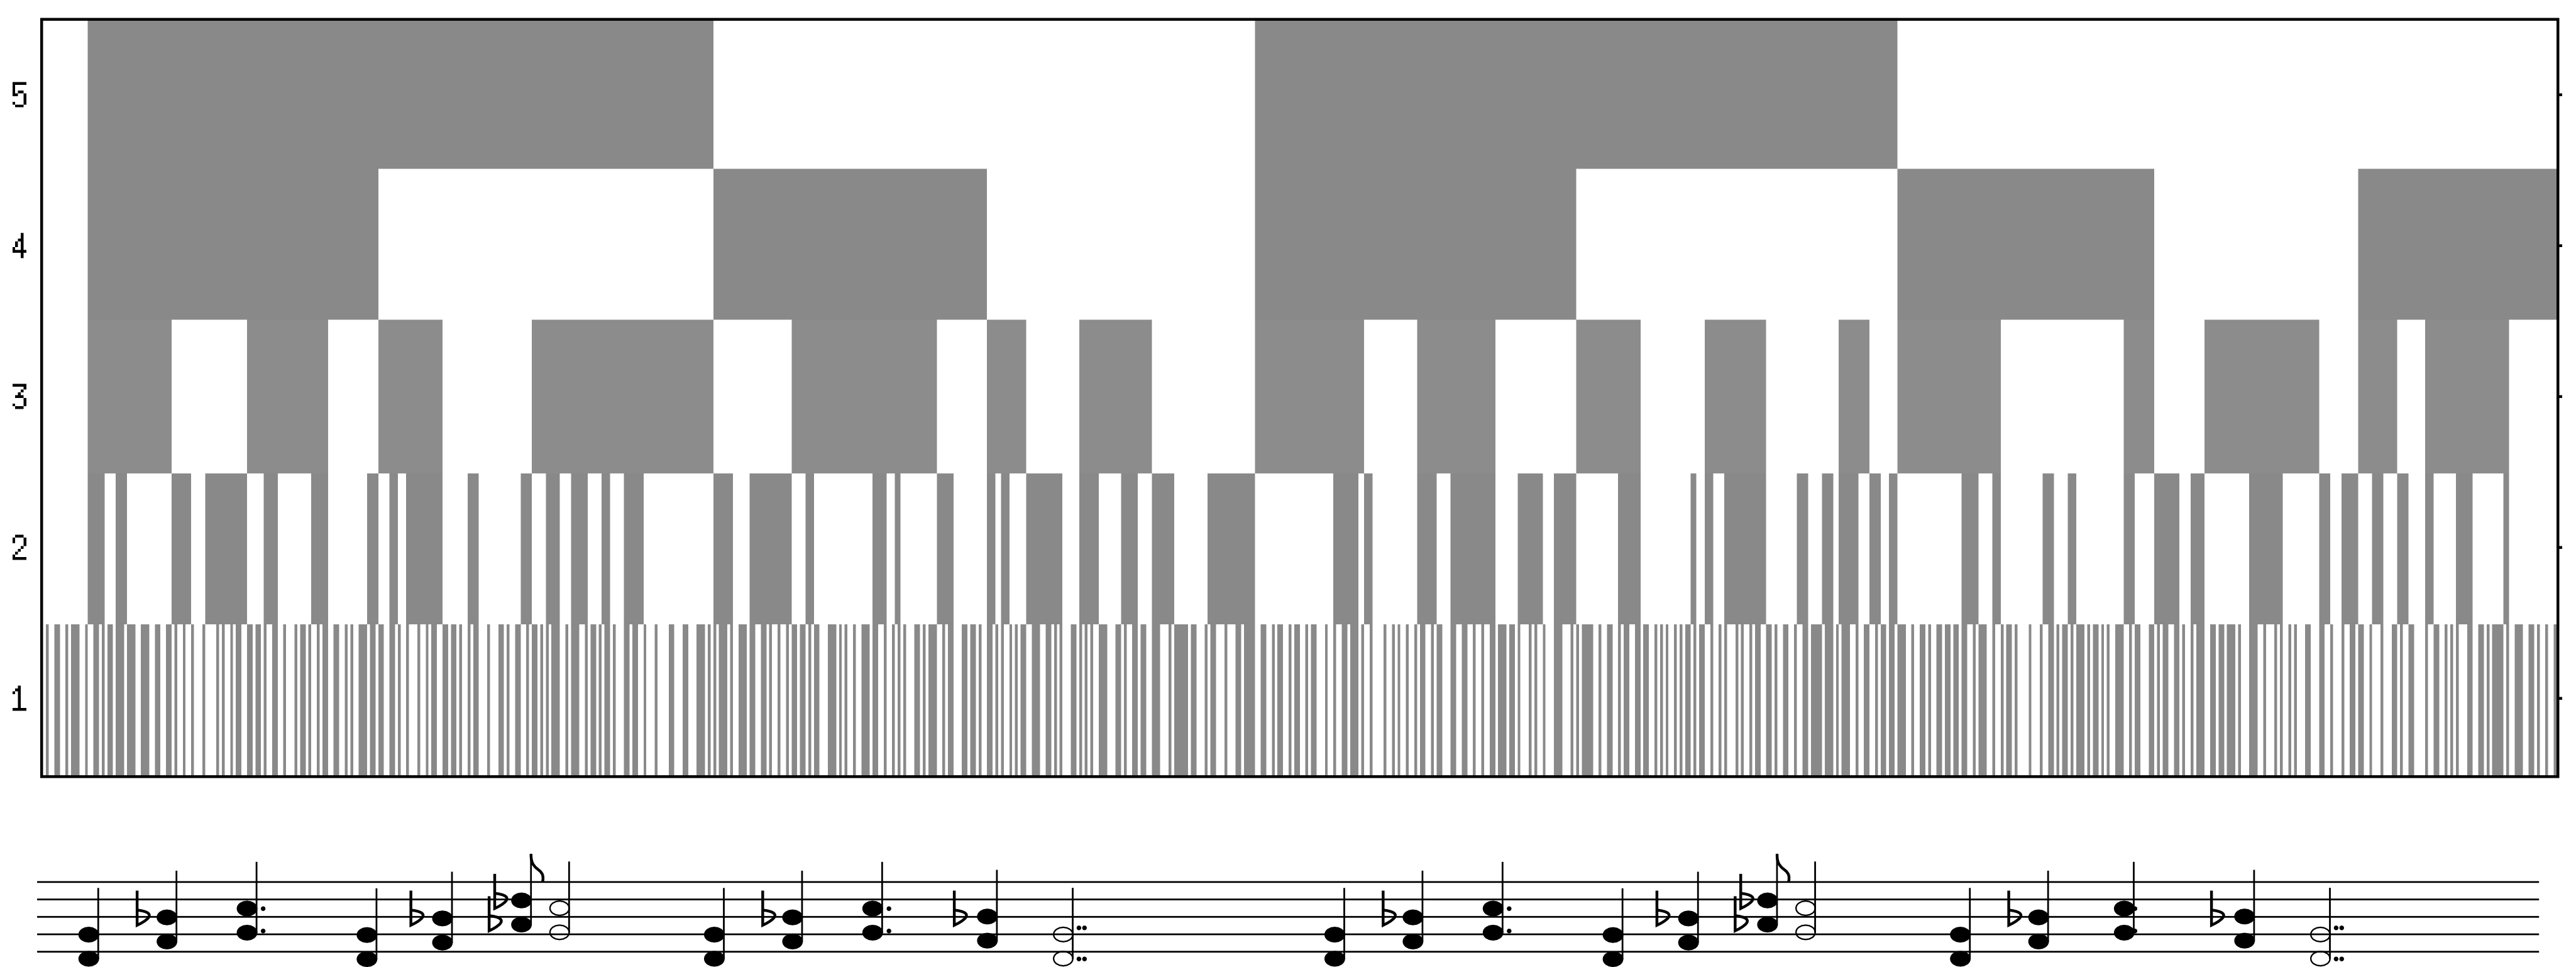
\includegraphics[width=\textwidth]{figures/smokeCrop}
           \caption{Segmentation du morceau de Deep Purple \emph{Smoke on the Water} (\emph{Machine Head}, Purple Records / EMI, 1972).}  \label{fig:smoke}
\end{figure}


  \section{ \nmu La  synthèse pour l'écoute artificielle} \label{sec:dcase}

  Ces travaux ont également été pour moi l'occasion de réfléchir au protocole d'évaluation, et en particulier aux données utilisées pour évaluer les algorithmes proposés. Il est évident que les données, qu'elles soient celles que l'on observe où celles que l'on cherche à prédire, constituent le fondement des sciences des données. Cette question est donc cruciale.

  Dans le domaine du traitement du signal, on fait souvent la différence entre des signaux dits \og réels \fg et des signaux dits \og synthétiques \fg. Les signaux réels sont issus d'un processus d'acquisition, plus ou moins maîtrisé, on parle souvent aussi de données brutes. La seule manipulation que l'on puisse alors faire pour mieux contrôler ces données, c'est de réduire la taille du corpus. Cette réduction peut se faire selon les différents axes de structuration. Dans le cas d'un corpus structuré sous forme de classes par exemple, on peut choisir de supprimer une ou plusieurs classes, ou de supprimer des éléments dans chaque classes de manière à obtenir un corpus équilibré, \textit{i.e.} avec un même nombre d'éléments par classe. Elle peut se faire également de manière globale, pour enlever des données aberrantes par exemple. Dans tout les cas, il est important de considérer que ces procédures sont délicates car difficile à motiver. Le risque du \og cherry picking \fg, qui consiste à trouver les données qui fonctionnent bien avec l'approche algorithmique défendue est toujours présent.

  \marginnote{Je n'évoquerai pas ici la question importante de la représentativité du corpus et de la division du corpus complet en corpus d'entrainement, de test, et de validation. Le lecteur peut se référer à l'excellent cours de Stéphane Mallat sur la notion de risque en apprentissage pour une approche formalisée de ce sujet. \\ Vidéos : \url{https://www.college-de-france.fr/site/stephane-mallat}\\
  Notes : \url{https://www.di.ens.fr/~mallat/CoursCollege.html}}.

  Les signaux synthétiques sont, eux, totalement contrôlés. Un modèle de signal est une méthode d'estimation des paramètres de ce modèle sont proposés. Et, en utilisant ce modèle de signal pour générer des exemples, on montre que la méthode d'estimation est effective sur ces exemples. Cela permet de faire une démonstration de faisabilité du modèle, mais n'est pas suffisante pour démontrer l'applicabilité de ce modèle à des problématiques concrètes.

  La méthode couramment prise est donc d'estimer ce niveau d'applicabilité en considérant les performances obtenues par le système en considérant des données brutes. Le principal risque de cette foi aveugle dans les résultats obtenus en utilisant les données brutes, est précisément que nous disposons souvent d'un contrôle très faible sur ces données, et ce qui à permis de les obtenir, \textit{i.e.} le processus d'acquisition pour les données observées, le processus d'annotation pour les données que l'on cherche éventuellement à prédire, etc.

  Prenons l'exemple du calcul d'une statistique telle que la moyenne, un ensemble d'outil nous permet de valider la pertinence de cette statistique, distribution, écart à la médiane, quartiles, etc. Pour un modèle avec plusieurs millions de paramètres libres comme c'est le cas pour les architectures de traitement de l'information telles que les réseaux de neurones profonds, les outils d'inspection sont nettement plus ardu à mettre en place. La valeur de la métrique de qualité obtenue par le système doit donc être appréciée avec beaucoup plus de mesure.

  Le modèle proposé est-il pertinent ? Est ce que l'information captée par la méthode d'estimation se rapporte à des phénomènes d'intérêts ? Pour tout problème qui sort de la trivialité, nous ne disposons pas à l'heure actuelle d'outils qui permettent de répondre à ces questions. Dans une forme moderne incluant la notion de recherche reproductible comme celle développée dans la section dédiée à \ref{sec:pairs}, l'inspection par les pairs constitue probablement la seule approche efficace à l'heure actuelle. Précisons ce propos avec deux exemples.

  La communauté d'acoustique environnementale se base principalement sur l'étude de mesures de niveaux acoustiques. De nombreuses études issues de cette communauté montrent que ces mesures ont leurs limites\cite{lavandier2006contribution} et qu'il serait utile de pouvoir décrire plus finement l'environnement sonore. De ce fait, une étude utilisant des techniques d'apprentissage montrait qu'il est possible de prédire le type d'environnement sonore urbain (rue, parc, boulevard, ...) avec une excellente précision\cite{aucouturier2007bag} a été très bien reçue par la communauté et pris pour fait acquis, en partie parce que cette étude appliquait des techniques mal connues par les membres de cette communauté.

  Intrigué par ces excellent résultats qui contrastaient avec des résultats obtenus dans d'autres études, j'ai entrepris de répliquer ces travaux. Cette tentative de réplication, effectuée en collaboration avec les auteurs, à été fructueuse et m'a permis de comprendre que les bons résultats obtenus étaient dus au protocole expérimental\cite{lagrange2015}. Les scènes présentes dans le corpus ont été enregistrées durant une période longue (environ une heure) et découpées en tronçons d'une minute. Etant donné la stationnarité de ce type de scènes sonores en terme de composition, deux tronçons successifs sont la plupart du temps quasiment identiques en terme de contenu. Le protocole expérimental n'empêchant pas que l'algorithme d'apprentissage exploite des tronçons d'une scène donnée pour prédire le label d'un tronçon de cette même scène, le problème s'en trouvait, dans son incarnation numérique, considérablement simplifié. \footnote{Ce phénomène est similaire à l'effet \og album \fg en musique. Les conditions d'enregistrements (microphones, mixage, mastering) sont souvent spécifique à l'album enregistré, spécificité que les algorithmes d'apprentissage exploitent pour minimiser leur erreur de prédiction. Pour mitiger cet effet, il convient alors de ne pas permettre d'avoir des chansons d'un même album dans les corpus d'apprentissage et de test.}.

  Prenons un second exemple. Le scattering d'ondelettes, un modèle de signal d'intérêt présenté dans la section dédiée aux représentations \nameref{sec:tfm}, a notamment été utilisé dans le cadre de la classification de genre musical\cite{anden2014deep}. Le scattering est en charge de produire une représentation du signal sonore qui soit informative mais de faible dimensionalité. Cette représentation est ensuite utilisé par algorithme de classification supervisée chargé de prédire à quel genre musical le morceau analysé appartient parmi une typologie déterminé.

  Dans une étude de réplication et d'analyse de la robustesse de ce système de prédiction du genre musical\cite{rodriguez2016analysing}, Rodriguez et Sturm montrent que les bonnes performances des méthodes de l'état de l'art se basent (au moins en partie) sur 1) une base de données mal structurée, et 2) la disponibilité d'information coïncidentes inaudible pour l'être humain.

  La base de données GTZAN proposée par George Tzanetakis a longtemps été une référence sur le sujet, car elle a été conçue pour évaluer le premier système de prédiction du genre musical\cite{tzanetakis2002musical}. Plusieurs études ont montrées les limites de cette base de données en terme de structure. L'utilisation d'une version plus robuste de la base fait décroitre les performances des méthodes testées de plus de 20 \%. Egalement, l'étude montre que des informations présentes dans les bandes de fréquences inférieures à 20 Hz sont déterminantes pour la qualité de la prédiction. En effet, en considérant une version où les bandes fréquences de fréquence inférieures à 20Hz sont fortement atténuées, les performances se réduisent de 15 \% environ. L'oreille ne percevant pas les signaux en dessous de 50 Hz, on peut dire que le système d'apprentissage se focalise sur des composantes inaudibles pour l'être humain.

  Ces deux exemples montrent combien il est difficile d'apprécier la performance d'un algorithme de traitement de données. Dans une posture particulièrement sceptique, Bob Sturm désigne tout ces algorithmes comme des potentiels "horses"  \marginnote{    
\includegraphics[width=.3\textwidth]{figures/hans}

Clever Hans était un cheval supposément capable de compter. Une personne lui donnait une opération mathématique à résoudre, et Hans tapait du sabot au sol et s'arrêtait de taper quand le compte de coups de sabot correspondait à la solution de l'opération. Confronté par un protocole rigoureux, il s'est avéré que Hans n'était capable de donner la bonne réponse que si la personne qui lui posait la question connaissait la réponse. En ce sens, Hans faisait preuve d'une intelligence sensible extrêmement fine pour pouvoir détecter les subtiles modifications de posture à l'approche du bon nombre de coups de sabots qui indiquait à Hans l'approche de sa récompense, mais cette intelligence n'était assurément pas de type mathématique.}.

  Néanmoins, le fait d'utiliser une corrélation fortuite entre différentes informations présentes dans les données, n'est pas nécessairement dommageable. Il est également extrêmement courant d'optimiser une fonction de coût donnée que l'on estime, pour des raisons axiomatiques concernant le type des données, ou empiriques. fonction de coût que l'on suppose corrélée avec l'objectif principal (prédire sur de nouvelles données, séparer des sources, ...). Dans la mesure où ces choix sont assumés, on en connaît mieux les limites. Il est par contre fondamental d'avoir conscience de ces problématiques pour être à même d'apprécier avec un regard suffisamment critique les mesures de performance dérivées de tel ou tel algorithme ou protocole expérimental\cite{lagrangehal-01635373}. Par exemple, une technique classique lors de l'optimisation consiste à procéder à l'"early stop", c'est-à-dire ne pas optimiser jusqu'à convergence de la fonction de coût optimisée, mais jusqu'à un certain nombre d'itérations correspondant au maximum de la fonction objectif.

  On a donc vu que l'usage de données synthétiques ne permettait qu'une validation du concept, et que l'usage de données brutes doit être encadrée avec soin et que, même si le but d'un algorithme de traitement de données est d'être capable \textit{in fine} de traiter des données brutes, le niveau de contrôle est extrêmement faible, ce qui réduit drastiquement la confiance que l'on peut avoir des métriques de performance obtenues. Je n'évoquerai pas ici le problème de l'annotation des données brutes qui se pose également, et qui, dans le cas de certaines tâches peut s'avérer particulièrement problématique. Deux exemples permettront d'appréhender ces difficultés :
\begin{enumerate}
  \item  Comment déterminer le genre musical d'un morceau de musique comme \og Psyché Rock \fg de Pierre Henry ?
  \item Comment annoter la fin d'un évènement sonore dans une scène sonore polyphonique ?
\end{enumerate}

  Dans le but de mitiger ces problèmes, il semble convenable de complémenter ces deux approches par une approche intermédiaire en considérant ce que j'appellerai des données \og simulées \fg. On verra dans la suite que, même si ces données simulées ne constituent pas une validation en soi, elles sont un outil particulièrement efficace pour une approche méthodologique de conception algorithmique mieux contrôlée et plus propice à être fondée sur un questionnement scientifique.

  Prenons le cas de la tâche de détection d'évènements sonores dans des scènes sonores complexes. Ces scènes sonores sont composées d'évènements sonores qui peuvent être présent de manière simultanés ou non, un bruit de fond plus ou moins élevé est présent. On souhaite que le système soit capable :
  \begin{enumerate}
    \item d'être robuste à la présence du bruit de fond, \textit{i.e.} ne pas détecter d'évènements quand il n'y a que du bruit de fond dans l'intervalle d'observation et ne pas se tromper de classes d'évènements lorsque le bruit de fond se superpose avec l'évènement  dans l'intervalle d'observation;
    \item d'être capable de gérer la diversité intra classe de chaque classe d'évènements sonores et de type de bruit de fond,  \textit{i.e.} dans le cas de la classe \og frappe sur clavier d'ordinateur \fg, le système doit être capable de gérer une grande diversité de marques de claviers et de style de frappes;
    \item être robuste aux changements de conditions d'enregistrements,  \textit{i.e.} le type de microphone, la qualité de l'enregistrement et les propriétés de réverbération de la pièce doivent pouvoir changer sans influer sur les performances du système.
  \end{enumerate}

  Evaluer ces éléments nécessite d'avoir à disposition des corpus séparés avec, dans le premier cas, un niveau de bruit de fond qui augmente, dans le deuxième cas, une diversité qui varie, et dans le troisième cas des conditions d'enregistrements qui changent. Bien entendu, la prise de son et l'annotation de scènes sonores brutes pour chacune de ces conditions expérimentales est possible mais particulièrement difficile et coûteux à mettre en place pour obtenir le niveau de précision souhaité.

  Nous avons considéré un modèle de scènes sonores qui permet d'aisément contrôler ces paramètres\marginnote{Une implantation de ce modèle dédiée à l'évaluation a été réalisée en Matlab \url{https://bitbucket.org/mlagrange/simscene}. Un outil alternatif a été développé en Python par Justin Salamon \url{https://github.com/justinsalamon/scaper}.}. Le modèle proposé se présente comme suit. Pour une scène $s$ composée de $z$ classes de sons, on a :

  \begin{equation}
  s(n)=\sum_{i=1}^{z}p_i(n)
  \end{equation}

  avec $n$ un indice temporel discret, et $p_i$ la piste correspondant à la classe $c_i$. La classe $c_i$ est composée de $\vert c_i\vert$ échantillons $c_{i,m}$, $1<m<\vert c_i\vert$.

  Soit $\mathcal{U}(x,y)$, une distribution uniforme d'entiers allant de $x$ à $y$, avec $x<y$. On définit $E_j^i$ ($j=\lbrace 1,2,\ldots,k_i\rbrace$) une suite de variables aléatoires indépendantes et identiquement distribuées (iid) suivant la loi $\mathcal{U}(1,\vert c_i \vert)$.

  \begin{equation}
  E_j^i \textrm{ iid : } \mathcal{U}(1,\vert c_i \vert) \quad \forall j
  \end{equation}

  Une piste $p_i$ est vue comme une séquence de $k_i$ échantillons d'événements. On définit $e_j^i(n)$, un événement choisi aléatoirement parmi les $\vert c_i\vert$ échantillons de la classe $c_i$ :

  \begin{equation}
  e_j^i=c_{i,E_j^i}
  \end{equation}

  On définit $V^i_j$ et $T^i_j$ ($j=\lbrace 1,2,\ldots,k_i\rbrace$), deux suites de variables aléatoires iid. Pour chaque piste $p_i$, les $V^i_j$ sont les facteurs de volume appliqués aux événements $e_j^i$, dont nous modélisons la distribution, par souci de simplicité, par une loi normale de moyenne $\mu_v^i$ et de variance $\sigma_v^i$. De même, pour chaque piste $p_i$, les $T_j^i$ sont les espacements inter-\emph{onsets}, lesquels suivent une loi normale de moyenne $\mu_t^i$ et de variance $\sigma_t^i$.

  Soit $\mathcal{N}(\mu,\sigma)$, une distribution normale de moyenne $\mu$ et de variance $\sigma$, on a alors :

  \begin{equation}
  \label{eq:ch4_eq1}
  V_j^i \textrm{ iid : } \mathcal{N}(\mu_a^{i},\sigma_a^{i}) \quad \forall j \quad \textrm{ et } \quad T_j^i \textrm{ iid : } \mathcal{N}({\mu_t^{i},\sigma_t^{i}}) \quad \forall j
  \end{equation}

  Lors de la génération d'une scène, les valeurs des $V^i_j$ et $T_j^i$ sont déterminées par tirage aléatoire, suivant les distributions correspondantes.

  On définit $d^i$ et $f^i$ les indices temporels de début et de fin de chaque piste $p_i$ respectivement.

  Une piste $p_i$ se définit alors comme suit:

  \begin{equation}
  \label{eq:ch4_eq2}
  p_{i}(n)= \sum_{j=1}^{k_i} V_j^i e_j^i(n-n_j^i) \quad \textrm{ avec } \quad n_j^i=n_{j-1}^i + T_j^i
  \end{equation}

  où, par convention, $n^i_0=d^i$ et $p_i(n)=0$ si $n>f^i$.

  Les paramètres du modèle sont, $\mu_v^i$, $\sigma_v^i$, $\mu_t^i$, $\sigma_t^i$, $d^i$ et $f^i$, et doivent être fixés pour chaque piste $p_i$. % La figure~\ref{fig:modelSequence} offre une illustration de l'action des paramètres introduits.

  Pour les bruits de fonds, deux distinctions sont à observer avec le modèle défini précédemment :

  \begin{enumerate}
  \item afin d'éviter toute sensation de discontinuité, deux échantillons de texture sont concaténés en considérant un recouvrement fixé, sur lequel est appliqué un fondu enchaîné (\emph{cross-fade}) à valeur d'énergie constante entre les échantillons, afin de réduire les discontinuités;
  \item il n'y a qu'un facteur de volume par piste ($V^i \textrm{ : } \mathcal{N}(\mu_v^{i},\sigma_v^{i})$), sa valeur s'appliquant à tous les échantillons.
  \end{enumerate}

  % \begin{figure}[t]
  %         \def\svgwidth{\linewidth}
  %         \input{figures/controlParameters2.pdf_tex}
  %        \caption{Représentation schématisée des pistes du modèle de scènes sonores.}\label{fig:modelSequence}
  % \end{figure}

  Nous avons mis en application ce modèle dans la première édition du challenge dcase, pour "detection and classification of acoustic scenes and events". Ce challenge, soutenu par la société IEEE ASSP, se propose de promouvoir l'activité scientifique et technique autour de la détection d'évènements et la classification de scènes dans un contexte sonore environnemental. Nous avons proposé dans ce cadre une tâche de détection d'évènements sonores se basant sur l'approche par simulation, à partir d'un corpus de scènes simulées grâce à l'outil simScene. Ce corpus utilisait des échantillons sonores et des bruits de fonds enregistrés à l'université de Queen Mary (qmul). Ce corpus sera nommée \emph{testQ}. Plusieurs laboratoires ont soumis leurs algorithmes, qui ont été transmis aux organisateurs qui se sont chargés de calculer les prédictions de ces algorithmes sur les données de test gardées secrètes lors du déroulement du challenge.

  Ces résultats ont été publiés\cite{stowellhal-01253912}. Nous avons ensuite voulu tester la capacité de généralisation de ces algorithmes, \textit{i.e.}~leur aptitude à maintenir des performances de détection similaires sur plusieurs corpus de scènes présentant des conditions expérimentales différentes. Pour ce faire, nous avons considéré un autre corpus d'échantillons sonores et de bruits de fonds  cette fois ci enregistrés à l'irccyn, Nantes pour générer de nouvelles scènes de test. Avec la permission des auteurs des différents systèmes soumis au challenge, ces derniers ont été évalués sur les corpus de scènes simulées, en utilisant les mêmes serveurs de calcul que ceux utilisés pour le challenge\footnote{De nombreuses métriques sont disponibles pour évaluer ce type de système. On se concentrera ici sur la métrique $Fcw_{eb}$, une F-mesure, calculée en prenant en compte les débuts des événements, et en normalisant les résultats par classe.}.

  La capacité de généralisation est considérée suivant trois angles :
  \begin{enumerate}
  \item robustesse à la diversité des échantillons: évaluer la capacité de généralisation sur des corpus de scènes possédant les mêmes caractéristiques structurelles (intensité sonore des échantillons, positionnement des échantillons), mais composés d'une sélection de échantillons différents.
  \item robustesse à la diversité structurelle: évaluer la capacité de généralisation sur des corpus de scènes composés des mêmes échantillons, mais dont les caractéristiques structurelles (intensité sonore des échantillons, positionnement/espacement moyen des échantillons) diffèrent;
  \item robustesse au niveau du bruit de fond. Ce niveau est mesuré en termes relatifs, avec la mesure ebr (pour \og event to background ratio \fg), exprimée en déciBels.
  \end{enumerate}

  Dans le premier cas, on considère une structure de scène de référence (correspondant aux annotations effectuées sur \emph{testQ} pour générer deux nouveaux corpus \emph{insQ}, et \emph{insI}. Le premier est généré à partir d'échantillons enregistrés à qmul, le second à partir d'échantillons enregistrés à l'irccyn. Le premier ayant une structure et un contenu sonore équivalent à \emph{testQ}, une certaine équivalence des performances est attendue. Comme on peut le voir sur la Figure \ref{fig:irccyn} c'est globalement le cas, sauf pour deux méthodes qui se retrouvent avec des performances drastiquement réduites.Une analyse d'erreur a montrée que ces changements de comportements étaient dûs à des phénomènes de sur-apprentissage, ce qui nous permet de valider le protocole expérimental. Le second corpus (\emph{insI}) permet d'évaluer la capacité de généralisation aux types d'échantillons. On voit sur la Figure \ref{fig:irccyn} que, à l'exception du système SCS, tout les autres ne sont pas capable de généraliser et se retrouvent avec des performances équivalentes à l'algorithme de référence (\og Baseline \fg).

  Dans le deuxième cas, on considère le modèle de génération de scènes précédemment décrit pour générer deux corpus avec une certaine diversité structurelle. Le premier considère des échantillons enregistrés à qmul et le second à l'irccyn. Les paramètres du modèle ($\mu_a$, $\sigma_a$, $\mu_t$, $\sigma_t$, ...) sont estimés à partir des annotations du corpus \emph{testQ}. Les résultats montrent une faible dépendance des algorithmes à la structure temporelle des scènes analysées. Ce résultat est attendu car la majorité des algorithmes ont peu de modélisation des dépendances temporelles.

  Dans le troisième cas, on considère quatre corpus, avec la même structure temporelle, les mêmes échantillons sonores, mais avec un niveau relatif de bruit de fond différent. L'ebr varie de -12 dB à 6 dB, le niveau de référence (équivalent à celui mesuré sur le corpus \emph{testQ})  étant de 0 dB. Les résultats, affichés sur la Figure \ref{fig:ebr}, montrent une forte sensibilité au niveau d'ebr pour toute les systèmes, sauf pour le système SCS, doté d'un algorithme de gestion du bruit de fond particulièrement efficace\cite{lafayhal-01111381}.

  \begin{figure}[t]
  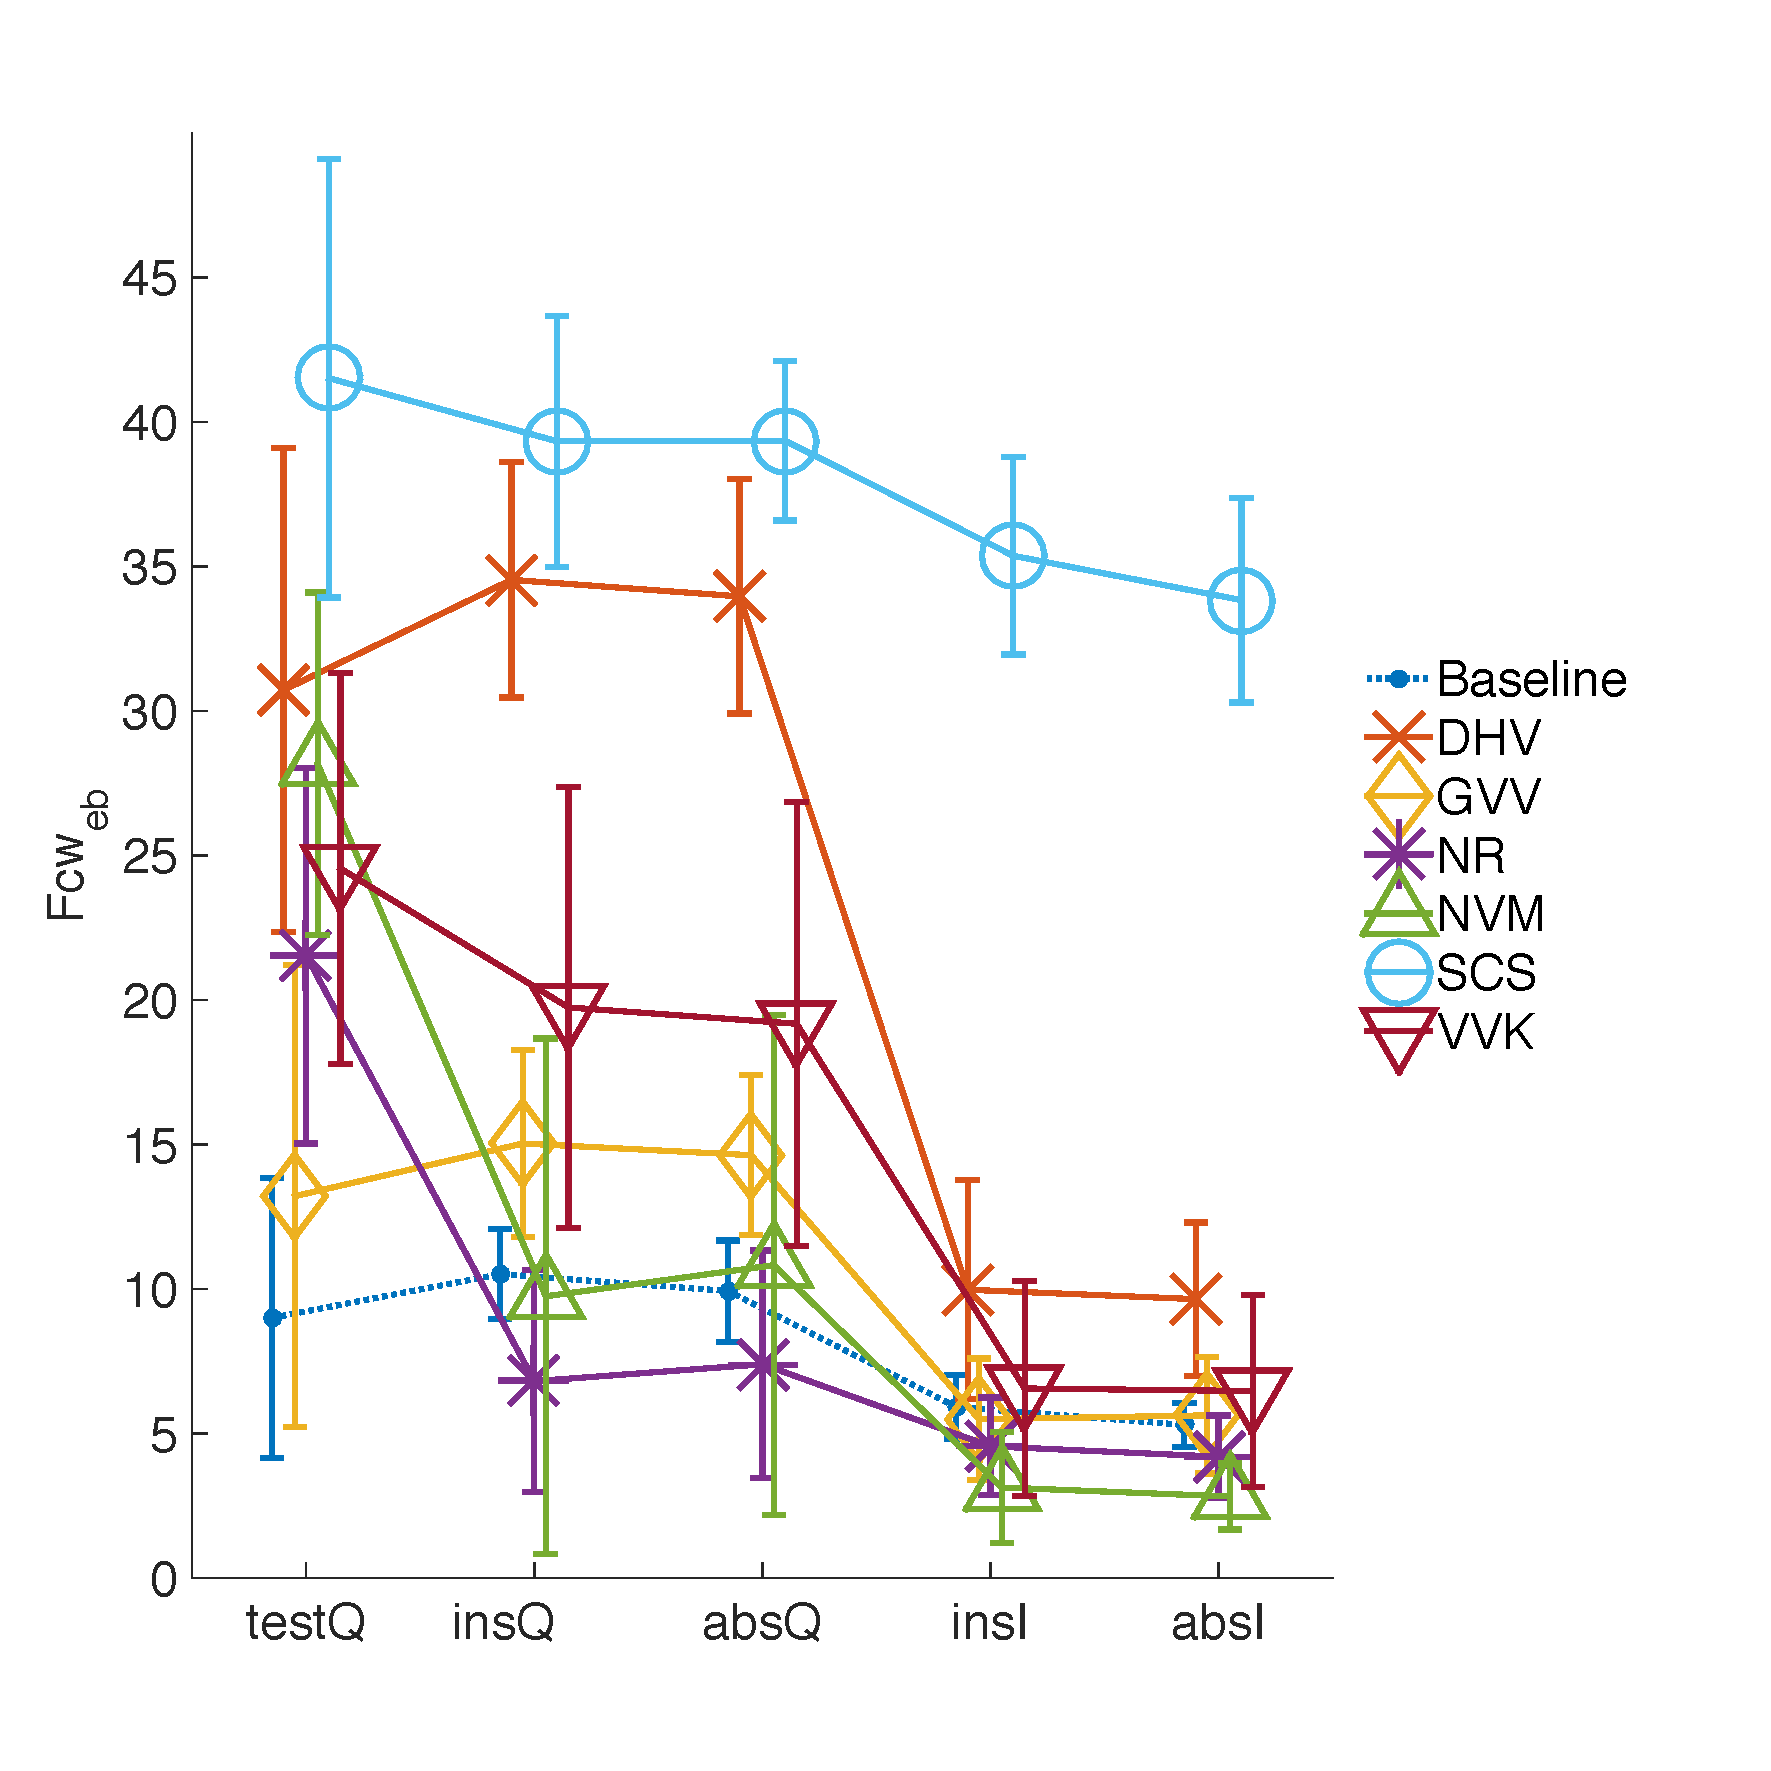
\includegraphics[width=\columnwidth]{dcase2013_1}
  \caption{Performances des systèmes évalués dans le cadre du challenge DCASE 2013 sur les corpus QMUL et IRCCYN en considérant la métrique $Fcw_{eb}$.}
  \label{fig:irccyn}
  \vspace{-4em}
  \end{figure}

  \begin{figure}[t]
  \begin{center}
  \includegraphics[width=\columnwidth]{dcase2013_2}
  \caption{Performances des systèmes évalués dans le cadre du challenge DCASE 2013 sur les corpus \emph{instance-QMUL} simulés avec différents $EBR$ ($6$, $0$, $-6$ et $-12dB$).}
  \label{fig:ebr}
  \end{center}
\vspace{-4em}
\end{figure}

  Notre implication dans le challenge dcase s'est confirmée en 2016\cite{mesa}, par la proposition d'une tâche similaire à celle proposée en 2013, avec quelques raffinements. Pour cette édition, nous souhaitions étudier l'influence de la répartition temporelle des évènement dans la scène, qui, dans le type de structures utilisées dans le l'édition de 2013 avait peu d'impact, probablement à cause d'une répartition assez parcimonieuse, sans recouvrement temporel entre les évènements. On distingue donc maintenant deux types de scènes, les scènes polyphoniques, scènes où les événements de différentes classes peuvent se recouvrir temporellement, et les scènes non-polyphoniques, scènes où un seul événement peut être actif à un moment donné.

  Au sein de ces deux types de scènes, deux paramètres sont considérés pour contrôler la simulation des scènes sonores : 1) le rapport moyen entre les niveaux des événements et du bruit de fond, et 2) le nombre d'événements présents pour chaque classe.

  Une analyse statistique des résultats\cite{lafayhal-01635414} montre un impact non significatif de la polyphonie et de la densité d'évènements, les systèmes réagissant différemment à la modification de ces facteurs expérimentaux, chaque système ayant opté pour un compromis précision / rappel différent. L'influence du niveau sonore des évènements sonore par rapport au bruit de fond est par contre elle significative. Ce dernier résultat indique qu'il est capital, afin d'améliorer les performances des algorithmes, de proposer des systèmes de gestion du bruit efficaces.

  Je terminerai cette section par des éléments de réflexion que j'ai amené lors du Workshop dcase 2018 où le constat était fait par une large communauté de chercheurs que les approches d'apprentissage profond et les méthodes ensemblistes appliquées à des classifieurs forts, apportent certes des performances élevées, mais finalement peu d'éléments de réflexion et compréhension.

  A mon avis, si la question posée est d'ordre pratique, ce n'est pas un problème que les réponses données ne soient que techniques\marginnote{Sans contraintes explicites, tout les moyens sont bons pour résoudre le problème.}. Comme nous en discuterons plus en détail dans le Chapitre dédié à \lnameref{chap:methode}, encore faut t'il que ces réponses aient un intérêt pour la communauté. Pour cela, la poursuite d'une méthode rigoureuse d'investigation reste d'importance (protocole expérimental approprié, précision du rapport, publication du code, réplicabilité, ...).

  Ceci ne doit pas en revanche être confondue avec une approche d'investigation scientifique qui doit elle, avant tout se baser sur une question. De la question naît un corpus d'observations qui peut servir ensuite de base à l'investigation qui peut comporter une partie technique, mais cela reste au service d'un questionnement qui lui est, par essence, scientifique. Il est donc du devoir de celui qui propose une tâche, si il y a lieu, de réfléchir à la pertinence de cette tâche au vu d'un certain questionnement scientifique pertinent pour la communauté.

  \section{ \nmu La  synthèse pour la psychologie expérimentale} \label{sec:psycho}

  Ces travaux nous ont amenés à écouter une grande nombre de scènes simulées, et à notre grande surprise, ce matériau sonore destiné finalement à n'être écouter que par des machines, s'est révélé particulièrement crédible en terme de qualité d'écoute. Ceci nous a amener à nous questionner sur la pertinence de ce type de stimuli pour nourrir des études de psycho perception.

  Par ce biais, j'ai eu le plaisir de contribuer au domaine de la psychologie expérimentale, en collaboration avec Grégoire Lafay et Nicolas Misdariis. Nous avons souhaités questionner la notion d'agrément sonore en zone urbaine, sujet d'une grande importance sanitaire.

  Pour cela, le modèle de scènes décrit précédemment, de part son réalisme et sa simplicité de manipulation s'est révélé être un outil pertinent pour questionner d'une nouvelle manière des notions comme l'agrément sonore. L'étude de référence sur le sujet de l'agrément sonore en zone urbaine\cite{guastavino2006ideal} considère un paradigme expérimental classique fondé sur la description faite par le sujet de l'objet d'étude. Chaque sujet est invité à verbaliser les propriétés d'un environnement sonore idéal ou non idéal. Ces descriptions textuelles sont ensuite traitées par une analyse psycho linguistique, des invariants dans les descriptions données par les sujets sont dégagés qui permettent alors de conclure quand aux propriétés de ces environnements.

  On note ici que ces environnements sont pensés par le sujet, puis décrit, ce qui place l'étude dans de la cadre de la théorie classique de la cognition, à savoir que les percepts subissent une étape de transduction en informations amodales que l'on peut alors questionner par le langage. Des théories alternatives existent, comme la théorie ancrée\cite{barsalou2010grounded} dont le propos est de ne pas distinguer perception et cognition en terme d'objets manipulés, mais en terme d'objectifs. Elle met à ce titre l'accent sur le contexte et la notion d'expérience, d'"embodiement". Dans cette théorie, les percepts sont le fondement, la matière brute des constructions cognitives qui en découlent. La cognition n'est plus en charge d'une transduction mais d'une extraction d'invariants qui serviront à construire des représentations de plus en plus abstraite.

  Notre proposition s'inscrit dans ce schéma de pensée, en demandant non plus au sujet de verbaliser son image mentale mais de \og construire \fg une représentation de l'image mentale que le sujet a d'un environnement sonore idéal\marginnote{Les scènes produites par les sujets sont disponibles \url{http://soundthings.org/research/urbanSoundScape/XP2014}.}. Comme on peut s'en rendre compte à l'écoute, de telles scènes sont plausibles mais ne sont pas pour autant réalistes au sens stricte du terme. On notera que l'on cherche ici, et ce avec un certain nombre de contraintes (durée de la scène, choix des éléments de base, paradigme de séquencement), en quelque sorte à exemplifier ces images mentales de haut niveau. Sans parler de caricatures, le côté pittoresque des scènes produites, notamment pour les scènes idéales, inscrit donc bien le protocole proposé dans la théorie ancrée de la perception.

  Cette étude a permis de confirmer certains résultats obtenus dans l'étude de Guastavino\cite{guastavino2006ideal} et d'en questionner d'autres. On citera par exemple, la présence systématique des bus dans les scènes idéales imaginées \og par écrit \fg, alors que notre étude les placent plutôt dans les scènes non idéales. On voit ici, comment d'un point de vue conceptuel, les transports en commun sont positivement connotés dans un environnement urbain, alors qu'ils restent des objets mobiles lourds avec une cylindrée conséquente, générant des niveaux de bruits mécaniques élevés\cite{lafayhal-01300399}.

  Au travers de ces deux exemples, on voit comment la capacité à manipuler la matière sonore nous permet de mieux questionner notre connaissance de la manière dont nous, humains, percevons et faisons sens de notre environnement. Le modèle présenté ici est à proprement parler un modèle de séquencement de sons, donc d'assez haut niveau. Nous étudierons dans le chapitre suivant les nombreux modèles de sons disponibles pour manipuler, dans la mesure de leur capacité, la matière sonore. %Je dédie donc la partie suivante à l'explicitation de ces propriétés qui nous guideront ensuite pour dresser un panorama des modèles de sons à notre disposition.


  %Mais ce n'est pas suffisant, nous devons disposer de modèles de sons qui soient capables de manipuler finement la matière sonore, et ce avec de bonnes propriétés. Je dédie donc la partie suivante à l'explicitation de ces propriétés qui nous guideront ensuite pour dresser un panorama des modèles de sons à notre disposition.
